\documentclass{cmspaper}
%
% LaTeX packages
%
\usepackage{graphicx}
%\usepackage{psfig}
%\usepackage{epsfig} 
%\addtolength{\topmargin}{0.5 in}
\usepackage{epic,rotating,epsfig}
\usepackage{amssymb}
\usepackage{amsmath}
\usepackage{pstricks,pst-grad}
\usepackage{subfigure}
\usepackage{lineno}
\usepackage{url}
\linenumbers



% include common commands
%-------------------------------------------------------------------------------
% private environments
%-------------------------------------------------------------------------------

\newcommand{\customChapter}[1]{\chapter{\boldmath #1 \unboldmath}}
\newcommand{\customSection}[1]{\section{\boldmath #1 \unboldmath}}
\newcommand{\customSubsection}[1]{\boldmath\subsection{#1}\unboldmath}
\newcommand{\customSubsubsection}[1]{\boldmath\subsubsection{#1}\unboldmath}

%-------------------------------------------------------------------------------
% technical reference definitions
%-------------------------------------------------------------------------------

\newcommand{\AppendixRef}[1]{Appendix~\ref{#1}}
\newcommand{\EquationRef}[1]{Equation~(\ref{#1})}
\newcommand{\FigureRef}[1]{Figure~\ref{#1}}
\newcommand{\ReferenceRef}[1]{Reference~\cite{#1}}
\newcommand{\SectionRef}[1]{Section~\ref{#1}}
\newcommand{\TableRef}[1]{Table~\ref{#1}}

%-------------------------------------------------------------------------------
% unit definitions
%-------------------------------------------------------------------------------

\newcommand{\fs}{\ensuremath{\mathrm{fs}}}
\newcommand{\ps}{\ensuremath{\mathrm{ps}}}
\newcommand{\ns}{\ensuremath{\mathrm{ns}}}
\newcommand{\ips}{\ensuremath{\mathrm{ps^{-1}}}}
\newcommand{\um}{\ensuremath{\mathrm{\mu m}}}
\newcommand{\mm}{\ensuremath{\mathrm{mm}}}
\newcommand{\cm}{\ensuremath{\mathrm{cm}}}
\renewcommand{\deg}{\ensuremath{^\mathrm{o}}}
\newcommand{\ifb}{\ensuremath{\mathrm{fb^{-1}}}}
\newcommand{\ipb}{\ensuremath{\mathrm{pb^{-1}}}}
\newcommand{\inb}{\ensuremath{\mathrm{nb^{-1}}}}
\newcommand{\iub}{\ensuremath{\mathrm{\mu b^{-1}}}}
\newcommand{\fb}{\ensuremath{\mathrm{fb}}}
\newcommand{\pb}{\ensuremath{\mathrm{pb}}}
\newcommand{\nb}{\ensuremath{\mathrm{nb}}}
\newcommand{\ub}{\ensuremath{\mathrm{\mu b}}}
\newcommand{\eV}{\ensuremath{\mathrm{e\kern -0.1em V}}}
\newcommand{\keV}{\ensuremath{\mathrm{ke\kern -0.1em V}}}
\newcommand{\MeV}{\ensuremath{\mathrm{Me\kern -0.1em V}}}
\newcommand{\GeV}{\ensuremath{\mathrm{Ge\kern -0.1em V}}}
\newcommand{\TeV}{\ensuremath{\mathrm{Te\kern -0.1em V}}}
\newcommand{\eVc}{\ensuremath{\mathrm{e\kern -0.1em V/}c}}
\newcommand{\keVc}{\ensuremath{\mathrm{ke\kern -0.1em V/}c}}
\newcommand{\MeVc}{\ensuremath{\mathrm{Me\kern -0.1em V/}c}}
\newcommand{\GeVc}{\ensuremath{\mathrm{Ge\kern -0.1em V/}c}}
\newcommand{\TeVc}{\ensuremath{\mathrm{Te\kern -0.1em V/}c}}
\newcommand{\eVcc}{\ensuremath{\mathrm{e\kern -0.1em V/}c^2}}
\newcommand{\keVcc}{\ensuremath{\mathrm{ke\kern -0.1em V/}c^2}}
\newcommand{\MeVcc}{\ensuremath{\mathrm{Me\kern -0.1em V/}c^2}}
\newcommand{\GeVcc}{\ensuremath{\mathrm{Ge\kern -0.1em V/}c^2}}
\newcommand{\TeVcc}{\ensuremath{\mathrm{Te\kern -0.1em V/}c^2}}
\newcommand{\Tesla}{\ensuremath{\mathrm{T}}}

\newcommand{\kB}{\ensuremath{\mathrm{kBytes}}}
\newcommand{\MB}{\ensuremath{\mathrm{MBytes}}}
\newcommand{\GB}{\ensuremath{\mathrm{GBytes}}}
\newcommand{\PB}{\ensuremath{\mathrm{PBytes}}}
\newcommand{\TB}{\ensuremath{\mathrm{TBytes}}}
\newcommand{\kBs}{\ensuremath{\mathrm{kBytes/s}}}
\newcommand{\MBs}{\ensuremath{\mathrm{MBytes/s}}}

\newcommand{\Hz}{\ensuremath{\mathrm{Hz}}}
\newcommand{\kHz}{\ensuremath{\mathrm{kHz}}}
\newcommand{\MHz}{\ensuremath{\mathrm{MHz}}}
\newcommand{\GHz}{\ensuremath{\mathrm{GHz}}}

\newcommand{\icmSQs}{\ensuremath{\mathrm{cm^{-2}s^{-1}}}}

%-------------------------------------------------------------------------------
% reconstruction variable definitions
%-------------------------------------------------------------------------------

\newcommand{\SQS}{\ensuremath{\sqrt{s}}}
\newcommand{\ILUM}{\ensuremath{{\cal L}}}
\newcommand{\TZ}{\ensuremath{t_0}}
\newcommand{\PHISIX}{\ensuremath{\mathrm{\phi_6}}}
\newcommand{\PHIZERO}{\ensuremath{\mathrm{\phi_0}}}
\newcommand{\DPHI}{\ensuremath{\mathrm{\Delta \phi}}}
\newcommand{\ETA}{\ensuremath{\mathrm{\eta}}}
\newcommand{\DZERO}{\ensuremath{\mathrm{d_0}}}
\newcommand{\DZEB}{\ensuremath{\mathrm{d_B}}}
\newcommand{\PT}{\ensuremath{\mathrm{p_T}}}
\newcommand{\Y}{\ensuremath{\mathrm{y}}}
\newcommand{\BDCUTS}{\ensuremath{\mathrm{\PT(\BD)>6\,\GeV;~|\Y| < 1}}}
\newcommand{\XSBD}{\ensuremath{\mathrm{\sigma_\BD}}}
\newcommand{\XSTOT}{\ensuremath{\mathrm{\sigma_{total}}}}

\newcommand{\Br}{\ensuremath{{\cal B}}}

%-------------------------------------------------------------------------------
% CKM matrix related
%-------------------------------------------------------------------------------

\newcommand{\LAM}{\ensuremath{\mathrm{\lambda}}}
\newcommand{\RHO}{\ensuremath{\mathrm{\rho}}}
%\newcommand{\ETA}{\ensuremath{\mathrm{\eta}}}

\newcommand{\VCKM}{\ensuremath{\mathrm{V}}}
\newcommand{\VCKMd}{\ensuremath{\mathrm{V^\dagger}}}

\newcommand{\VUD}{\ensuremath{\mathrm{V_{ud}}}}
\newcommand{\VUS}{\ensuremath{\mathrm{V_{us}}}}
\newcommand{\VUB}{\ensuremath{\mathrm{V_{ub}}}}
\newcommand{\VCD}{\ensuremath{\mathrm{V_{cd}}}}
\newcommand{\VCB}{\ensuremath{\mathrm{V_{cb}}}}
\newcommand{\VCS}{\ensuremath{\mathrm{V_{cs}}}}
\newcommand{\VTB}{\ensuremath{\mathrm{V_{tb}}}}
\newcommand{\VTD}{\ensuremath{\mathrm{V_{td}}}}
\newcommand{\VTS}{\ensuremath{\mathrm{V_{ts}}}}

\newcommand{\VUDs}{\ensuremath{\mathrm{V^*_{ud}}}}
\newcommand{\VUBs}{\ensuremath{\mathrm{V^*_{ub}}}}
\newcommand{\VCDs}{\ensuremath{\mathrm{V^*_{cd}}}}
\newcommand{\VCBs}{\ensuremath{\mathrm{V^*_{cb}}}}
\newcommand{\VCSs}{\ensuremath{\mathrm{V^*_{cs}}}}
\newcommand{\VTBs}{\ensuremath{\mathrm{V^*_{tb}}}}
\newcommand{\VTDs}{\ensuremath{\mathrm{V^*_{td}}}}
\newcommand{\VTSs}{\ensuremath{\mathrm{V^*_{ts}}}}

%-------------------------------------------------------------------------------
% physics parameter definitions
%-------------------------------------------------------------------------------

\newcommand{\EPS}{\ensuremath{\varepsilon}}
\newcommand{\DIL}{\ensuremath{\rm D}}
\newcommand{\EPSDSQ}{\ensuremath{\rm \varepsilon D^2}}

\newcommand{\SINTA}{\ensuremath{\sin 2 \alpha}}
\newcommand{\SINTB}{\ensuremath{\sin 2 \beta}}

\newcommand{\PHIDNP}{\ensuremath{\mathrm{\phi^d_{NP}}}}
\newcommand{\PHISNP}{\ensuremath{\mathrm{\phi^s_{NP}}}}

\newcommand{\FU}{\ensuremath{\mathrm{f_u}}}
\newcommand{\FD}{\ensuremath{\mathrm{f_d}}}
\newcommand{\FS}{\ensuremath{\mathrm{f_s}}}
\newcommand{\FLB}{\ensuremath{\mathrm{f_{\Lambda_B}}}}
\newcommand{\EPSB}{\ensuremath{\varepsilon_\mathrm{b}}}

\newcommand{\GBS}{\ensuremath{\Gamma_s}}
\newcommand{\DGBS}{\ensuremath{\Delta \Gamma_s}}
\newcommand{\MBS}{\ensuremath{m_\BS}}
\newcommand{\DMS}{\ensuremath{\Delta m_s}}
\newcommand{\XS}{\ensuremath{x_s}}

\newcommand{\GBD}{\ensuremath{\Gamma_\mathrm{d}}}
\newcommand{\DGBD}{\ensuremath{\Delta \Gamma_\mathrm{d}}}
\newcommand{\DG}{\ensuremath{\Delta\Gamma}}
\newcommand{\DGG}{\ensuremath{\Delta\Gamma/\Gamma}}
\newcommand{\DGGS}{\ensuremath{\Delta\Gamma_s/\Gamma_s}}
\newcommand{\MBD}{\ensuremath{m_d}}
\newcommand{\DMD}{\ensuremath{\Delta m_d}}
\newcommand{\XD}{\ensuremath{x_d}}

\newcommand{\MT}{\ensuremath{m_t}}

%-------------------------------------------------------------------------------
% particle definitions
%-------------------------------------------------------------------------------

% single particles - bosons
\newcommand{\GAM}{\ensuremath{\gamma}}
\newcommand{\Z}{\ensuremath{\mathrm{Z}}}
\newcommand{\W}{\ensuremath{\mathrm{W}}}
\newcommand{\WP}{\ensuremath{\mathrm{W^+}}}
\newcommand{\WM}{\ensuremath{\mathrm{W^-}}}
\newcommand{\WPM}{\ensuremath{\mathrm{W^\pm}}}
\newcommand{\WMP}{\ensuremath{\mathrm{W^\mp}}}
\newcommand{\Higgs}{\ensuremath{\mathrm{H}}}

% single particles - leptons
\newcommand{\EL}{\ensuremath{\mathrm{e}}}
\newcommand{\ELP}{\ensuremath{\mathrm{e^+}}}
\newcommand{\ELM}{\ensuremath{\mathrm{e^-}}}
\newcommand{\MU}{\ensuremath{\mathrm{\mu}}}
\newcommand{\MUP}{\ensuremath{\mathrm{\mu^+}}}
\newcommand{\MUM}{\ensuremath{\mathrm{\mu^-}}}
\newcommand{\LP}{\ensuremath{\ell^{+}}}
\newcommand{\LM}{\ensuremath{\ell^{-}}}
\newcommand{\NL}{\ensuremath{\nu_{\ell}}}
\newcommand{\NLB}{\ensuremath{\overline{\nu}_{\ell}}}

% single particles - quarks
\newcommand{\up}{\ensuremath{u}}
\newcommand{\down}{\ensuremath{d}}
\newcommand{\strange}{\ensuremath{s}}
\newcommand{\charm}{\ensuremath{c}}
\newcommand{\bottom}{\ensuremath{b}}
\newcommand{\topquark}{\ensuremath{t}}
\newcommand{\ubar}{\ensuremath{\bar{u}}}
\newcommand{\dbar}{\ensuremath{\bar{d}}}
\newcommand{\sbar}{\ensuremath{\bar{s}}}
\newcommand{\cbar}{\ensuremath{\bar{c}}}
\newcommand{\bbar}{\ensuremath{\bar{b}}}
\newcommand{\tbar}{\ensuremath{\bar{t}}}




% single particles - B hadrons
\newcommand{\B}{\ensuremath{B}}
\newcommand{\BU}{\ensuremath{\mathrm{B_u}}}
\newcommand{\BUP}{\ensuremath{\mathrm{B^+}}}
\newcommand{\BUM}{\ensuremath{\mathrm{B^-}}}
\newcommand{\BD}{\ensuremath{\mathrm{B^0}}}
\newcommand{\BDB}{\ensuremath{\mathrm{\overline{B^0}}}}
\newcommand{\BS}{\ensuremath{\mathrm{B_s}}}
\newcommand{\BSB}{\ensuremath{\mathrm{\overline{B}_s}}}
\newcommand{\BC}{\ensuremath{\mathrm{B_c}}}
\newcommand{\BCP}{\ensuremath{\mathrm{B_c^+}}}
\newcommand{\BCM}{\ensuremath{\mathrm{B_c^-}}}
\newcommand{\LB}{\ensuremath{\mathrm{\Lambda_b}}}
\newcommand{\LBB}{\ensuremath{\mathrm{\overline{\Lambda}_b}}}

% single particles - charmed hadrons
\newcommand{\D}{\ensuremath{D}}
\newcommand{\DZ}{\ensuremath{\mathrm{D^0}}}
\newcommand{\DZB}{\ensuremath{\mathrm{\overline{D}^0}}}
\newcommand{\DP}{\ensuremath{\mathrm{D^+}}}
\newcommand{\DM}{\ensuremath{\mathrm{D^-}}}
\newcommand{\DS}{\ensuremath{\mathrm{D_s}}}
\newcommand{\DSP}{\ensuremath{\mathrm{D^+_s}}}
\newcommand{\DSM}{\ensuremath{\mathrm{D^-_s}}}
\newcommand{\DSPM}{\ensuremath{\mathrm{D^\pm_s}}}
\newcommand{\DSMP}{\ensuremath{\mathrm{D^\mp_s}}}
\newcommand{\DSS}{\ensuremath{\mathrm{D^*_s}}}
\newcommand{\DSSP}{\ensuremath{\mathrm{D^{*\,+}_s}}}
\newcommand{\DSSM}{\ensuremath{\mathrm{D^{*\,-}_s}}}
\newcommand{\DSSPM}{\ensuremath{\mathrm{D^{*\,\pm}_s}}}
\newcommand{\DSSMP}{\ensuremath{\mathrm{D^{*\,\mp}_s}}}
\newcommand{\LC}{\ensuremath{\mathrm{\Lambda_c}}}
\newcommand{\LCP}{\ensuremath{\mathrm{\Lambda_c^+}}}
\newcommand{\LCM}{\ensuremath{\mathrm{\Lambda_c^-}}}
\newcommand{\SCZ}{\ensuremath{\mathrm{\Sigma_c^0}}}
\newcommand{\SCP}{\ensuremath{\mathrm{\Sigma_c^+}}}
\newcommand{\SCPP}{\ensuremath{\mathrm{\Sigma_c^{++}}}}

% single particles - quarkonia
\newcommand{\UPSI}{\ensuremath{\Upsilon}}
\newcommand{\JPSI}{\ensuremath{\mathrm{J/\psi}}}
\newcommand{\PHI}{\ensuremath{\phi}}

% single particles - kaons
\newcommand{\K}{\ensuremath{K}}
\newcommand{\KP}{\ensuremath{\mathrm{K^+}}}
\newcommand{\KM}{\ensuremath{\mathrm{K^-}}}
\newcommand{\KPM}{\ensuremath{\mathrm{K^\pm}}}
\newcommand{\KMP}{\ensuremath{\mathrm{K^\mp}}}
\newcommand{\KZ}{\ensuremath{\mathrm{K^0}}}
\newcommand{\KZB}{\ensuremath{\mathrm{\overline{K}^0}}}
\newcommand{\KS}{\ensuremath{\mathrm{K^*}}}
\newcommand{\KSZ}{\ensuremath{\mathrm{K^{*\,0}}}}
\newcommand{\KZS}{\ensuremath{\mathrm{K^0_S}}}
\newcommand{\KZL}{\ensuremath{\mathrm{K^0_L}}}
\newcommand{\LS}{\ensuremath{\mathrm{\Lambda}}}
\newcommand{\SSZ}{\ensuremath{\mathrm{\Sigma^0}}}
\newcommand{\SSP}{\ensuremath{\mathrm{\Sigma^{+}}}}
\newcommand{\SSM}{\ensuremath{\mathrm{\Sigma^{-}}}}

% single particles - pions
\newcommand{\PI}{\ensuremath{\pi}}
\newcommand{\PIZ}{\ensuremath{\pi^0}}
\newcommand{\PIP}{\ensuremath{\pi^+}}
\newcommand{\PIM}{\ensuremath{\pi^-}}

% single particles - protons
\newcommand{\PR}{\ensuremath{p}}
\newcommand{\PRB}{\ensuremath{\overline{p}}}

% particle pairs
\newcommand{\EE}{\ensuremath{e^+e^-}}
\newcommand{\PPBAR}{\ensuremath{p\overline{p}}}
\newcommand{\BBBAR}{\ensuremath{b\overline{b}}}
\newcommand{\CCBAR}{\ensuremath{c\overline{c}}}
\newcommand{\ZZ}{\ensuremath{\mathrm{Z^{0}Z^{0}}}}
\newcommand{\WW}   {\ensuremath{\WP\WM}}
\newcommand{\TTBAR}{\ensuremath{\mathrm{t}\bar{\mathrm{t}}}}

% more complicated particle combination
\newcommand{\WPlusJets}{\ensuremath{W\mathrm{+Jets}}}
\newcommand{\WPlusGamma}{\ensuremath{W\mathrm{+}\gamma}}
\newcommand{\Wb}{\ensuremath{Wb}}
\newcommand{\Wc}{\ensuremath{Wc}}
\newcommand{\Wbb}{\ensuremath{Wbb}}
\newcommand{\Wcc}{\ensuremath{Wcc}}

%-------------------------------------------------------------------------------
% particle decay chain definitions
%-------------------------------------------------------------------------------

% helper
\renewcommand{\to}{\ensuremath{\rightarrow}}

% Higgs decays
\newcommand{\HiggsToWW}   {\ensuremath{\Higgs \to \WPM\WMP}}


% Lambda_b hadronic decays
\newcommand{\LBPRDZPI}   {\ensuremath{\LB \to \PR \DZ \PIP}}
\newcommand{\LBLCDS}     {\ensuremath{\LB \to \LCP \DSM}}
\newcommand{\LBLCDSS}    {\ensuremath{\LB \to \LCP \DSSM}}
\newcommand{\LBLCDSPIPI} {\ensuremath{\LB \to \LCP \DSM \PIP \PIM}}
\newcommand{\LBLCDSSPIPI}{\ensuremath{\LB \to \LCP \DSSM \PIP \PIM}}
\newcommand{\LBPRDS}     {\ensuremath{\LB \to \PR \DSM}}
\newcommand{\LBPRDSS}    {\ensuremath{\LB \to \PR \DSSM}}
\newcommand{\LBPRDSPIPI} {\ensuremath{\LB \to \PR \DSM \PIP \PIM}}
\newcommand{\LBPRDSSPIPI}{\ensuremath{\LB \to \PR \DSSM \PIP \PIM}}
\newcommand{\LBLCPI}     {\ensuremath{\LB \to \LCP \PIM}}
\newcommand{\LBLCPIPIPI} {\ensuremath{\LB \to \LCP \PIM \PIP \PIM}}
\newcommand{\LBSCZPIPI}  {\ensuremath{\LB \to \SCZ \PIM \PIP}}
\newcommand{\LBSCPPPIPI} {\ensuremath{\LB \to \SCPP \PIM \PIM}}
\newcommand{\LBPRPI}     {\ensuremath{\LB \to \PR \PIM}}
\newcommand{\LBPRPIPIPI} {\ensuremath{\LB \to \PR \PIM \PIP \PIM}}
\newcommand{\LBPRK}      {\ensuremath{\LB \to \PR \KM}}

% Lambda_c hadronic decays
\newcommand{\LCPRKPI}   {\ensuremath{\LCP \to \PR \KM \PIP}}
\newcommand{\LCLSPIPIPI}{\ensuremath{\LCP \to \LS \PIP \PIM \PIP}}
\newcommand{\LCLSPI}    {\ensuremath{\LCP \to \LS \PIP}}

% Sigma_c hadronic decays
\newcommand{\SCZLCPI}   {\ensuremath{\SCZ \to \LCP \PIM}}
\newcommand{\SCPPLCPI}  {\ensuremath{\SCPP \to \LCP \PIP}}

% Bs hadronic decays
\newcommand{\BSDSPI}   {\ensuremath{\BS \to \DSM \PIP}}
\newcommand{\BSDSSPI}  {\ensuremath{\BS \to \DSSM \PIP}}
\newcommand{\BSDSTPI}  {\ensuremath{\BS \to \DSM \PIP \PIP \PIM}}
\newcommand{\BSDSSTPI} {\ensuremath{\BS \to \DSSM \PIP \PIP \PIM}}
\newcommand{\BSDSDS}   {\ensuremath{\BS \to \DSM \DSP}}
\newcommand{\BSDSSDS}  {\ensuremath{\BS \to \DSSPM \DSMP}}
\newcommand{\BSDSSDSS} {\ensuremath{\BS \to \DSSM \DSSP}}
\newcommand{\BSDSKPHI} {\ensuremath{\BS \to \DSPM \KMP \PHI }}
\newcommand{\BSDSSKPHI}{\ensuremath{\BS \to \DSSPM \KMP \PHI }}
\newcommand{\BSKK}     {\ensuremath{\BS \to \KM \KP}}
\newcommand{\BSKPI}    {\ensuremath{\BS \to \KM \PIP}}

% Bs leptonic decays
\newcommand{\BSJPSIPHI}{\ensuremath{\BS \to \JPSI \PHI}}
\newcommand{\BSNLDSX}  {\ensuremath{\BS \to \NL \LP \DSM X}}

% Bd hadronic decays
\newcommand{\BDPIPI}   {\ensuremath{\BD \to \PIM \PIP}}
\newcommand{\BDPIK}    {\ensuremath{\BD \to \PIM \KP}}
\newcommand{\BDJPSIKS} {\ensuremath{\BD \to \JPSI \KZS}}

% Ds* decays
\newcommand{\DSSDSGP}  {\ensuremath{\DSS \to \DS \gamma,\PIZ}}

% Ds decays
\newcommand{\DSPHIPI}  {\ensuremath{\DSM \to \PHI \PIM}}
\newcommand{\DSKSK}    {\ensuremath{\DSM \to \KSZ \KM}}
\newcommand{\DSPIPIPI} {\ensuremath{\DSM \to \PIM \PIP \PIM}}
\newcommand{\DSKZSK}   {\ensuremath{\DSM \to \KZS \KM}}
\newcommand{\DSTPI}    {\ensuremath{\DSM \to \PIM \PIM \PIP}}
\newcommand{\DSKKZSPIPI}{\ensuremath{\DSM \to \KP \KZS \PIM \PIM}}
\newcommand{\DSPHITPI} {\ensuremath{\DSM \to \PHI \PIM \PIM \PIP}}
\newcommand{\DSKPIPI}  {\ensuremath{\DSM \to \KM \PIM \PIP}}
\newcommand{\DSNLLPHIX}{\ensuremath{\DSM \to \NLB \LP \PHI   X}}
\newcommand{\DSALL}    {\ensuremath{\DSM \to \rm all \,\, above }}

% D decays
\newcommand{\DZKPI}    {\ensuremath{\DZ \to \KM \PIP}}
\newcommand{\DZKPIPIPI}{\ensuremath{\DZ \to \KM \PIP \PIM \PIP}}

% Lambda_c hadronic decays
\newcommand{\LSPRPI}   {\ensuremath{\LS \to \PR \PIM}}

% Phi decays
\newcommand{\PHIKK}    {\ensuremath{\PHI \to \KM \KP}}

% K* decays
\newcommand{\KSKPI}    {\ensuremath{\KSZ \to \KP \PIM}}

% Kshort decays
\newcommand{\KZSPIPI}  {\ensuremath{\KZS \to \KP \PIM}}

% ---------------------------------------------------------
% new commands for common use in HWW cms-not
% F.Stoeckli , 10-18-2007
%
% including Guillelmos commands from HWW.tex

\newcommand{\CLs}{\ensuremath{CL_\mathrm{s}}}
\newcommand{\CLb}{\ensuremath{CL_\mathrm{b}}}
\newcommand{\CLsb}{\ensuremath{CL_\mathrm{s+b}}}

\newcommand{\GeV}{\ensuremath{\mathrm{Ge\kern -0.1em V}}}
\newcommand{\TeVcc}{\ensuremath{\,\mathrm{Te\kern -0.1em V\!/c}^2}}
\newcommand{\GeVcc}{\ensuremath{\,\mathrm{Ge\kern -0.1em V\!/c}^2}}
\newcommand{\MeVcc}{\ensuremath{\,\mathrm{Me\kern -0.1em V\!/c}^2}}
\newcommand{\GeVc}{\ensuremath{\mathrm{Ge\kern -0.1em V}\!/c}}
\newcommand{\nanob}{\mbox{{\rm ~nb}~}}
\newcommand{\fb}{\ensuremath{\mathrm{fb}}}
\newcommand{\pb}{\ensuremath{\mathrm{pb}}}
\newcommand{\ifb}{\ensuremath{\mathrm{fb^{-1}}}}
\newcommand{\ipb}{\ensuremath{\mathrm{pb^{-1}}}}
\newcommand{\grad}{\ensuremath{^{\circ}}}
%
% Special user made math symbols
%
\newcommand{\lsim}{\raisebox{-1.5mm}{$\:\stackrel{\textstyle{<}}{\textstyle{\sim}}\:$}}
\newcommand{\gsim}{\raisebox{-1.5mm}{$\:\stackrel{\textstyle{>}}{\textstyle{\sim}}\:$}}

% particles

\newcommand{\pipm}{\ensuremath{\pi^{\pm}}}
\newcommand{\pizero}{\ensuremath{\pi^{0}}}
\newcommand{\Kpm}{\ensuremath{K^{\pm}}}
\newcommand{\Hi}{\ensuremath{\mathrm{H}}}
\newcommand{\W}{\ensuremath{\mathrm{W}}}
\newcommand{\Wt}{\ensuremath{\mathrm{Wt}}}
\newcommand{\Wstar}{\ensuremath{\mathrm{W}^{*}}}
\newcommand{\Wparenthesisstar}{\ensuremath{\mathrm{W}^{(*)}}}
\newcommand{\WW}{\ensuremath{\W\W}}
\newcommand{\Z}{\ensuremath{\mathrm{Z}}}
\newcommand{\Zstar}{\ensuremath{\mathrm{Z}^{*}}}
\newcommand{\ZZ}{\ensuremath{\Z\Z}}
\newcommand{\WZ}{\ensuremath{\W\Z}}
\newcommand{\E}{\ensuremath{\mathrm{e}}}
\newcommand{\Ep}{\ensuremath{\mathrm{e}^{+}}}
\newcommand{\Em}{\ensuremath{\mathrm{e}^{-}}}
\newcommand{\Epm}{\ensuremath{\mathrm{e}^{\pm}}}
\newcommand{\Emp}{\ensuremath{\mathrm{e}^{\mp}}}
\newcommand{\Mu}{\ensuremath{\mu}}
\newcommand{\Mup}{\ensuremath{\mu^{+}}}
\newcommand{\Mum}{\ensuremath{\mu^{-}}}
\newcommand{\Mupm}{\ensuremath{\mu^{\pm}}}
\newcommand{\Mump}{\ensuremath{\mu^{\mp}}}
\newcommand{\Tau}{\ensuremath{\tau}}
\newcommand{\Nu}{\ensuremath{\nu}}
\newcommand{\Nubar}{\ensuremath{\bar{\nu}}}
\newcommand{\Lep}{\ensuremath{\ell}}
\newcommand{\Lepp}{\ensuremath{\ell^{+}}}
\newcommand{\Lepm}{\ensuremath{\ell^{-}}}
\newcommand{\Lprime}{\ensuremath{\Lep^{\prime}}}
\newcommand{\Prot}{\ensuremath{\mathrm{p}}}
\newcommand{\Pbar}{\ensuremath{\bar{\mathrm{p}}}}
\newcommand{\PP}{\Prot\Prot}
\newcommand{\PPbar}{\Prot\Pbar}
\newcommand{\ttbar}{\ensuremath{\mathrm{t}\bar{\mathrm{t}}}}
\newcommand{\qq}{\ensuremath{\mathrm{q}\mathrm{q}}}
\newcommand{\bbbar}{\ensuremath{\mathrm{b}\bar{\mathrm{b}}}}
\newcommand{\Wtb}{\ensuremath{\W\mathrm{t}\mathrm{b}}}
\newcommand{\Top}{\ensuremath{\mathrm{t}}}
\newcommand{\Bot}{\ensuremath{\mathrm{b}}}
\newcommand{\Atop}{\ensuremath{\bar{\mathrm{t}}}}
\newcommand{\Abot}{\ensuremath{\bar{\mathrm{b}}}}
% arrow
\newcommand{\To}{\ensuremath{\rightarrow}}

% masses
\newcommand{\mHi}{\ensuremath{m_{\mathrm{H}}}}
\newcommand{\mW}{\ensuremath{m_{\mathrm{W}}}}
\newcommand{\mZ}{\ensuremath{m_{\mathrm{Z}}}}
\newcommand{\mll}{\ensuremath{m_{\Lep\Lep}}}


% kinematics
\newcommand{\pt}{\ensuremath{p_\mathrm{T}}}
\newcommand{\ptHat}{\ensuremath{\hat{p_\mathrm{T}}}}
\newcommand{\ptveto}{\ensuremath{\pt^\mathrm{veto}}}
\newcommand{\ptl}{\ensuremath{p_\perp^{\Lep}}}
\newcommand{\ptlmax}{\ensuremath{p_{\mathrm{T}}^{\Lep,\mathrm{max}}}}
\newcommand{\ptlmin}{\ensuremath{p_{\mathrm{T}}^{\Lep,\mathrm{min}}}}
\newcommand{\met}{\ensuremath{\Et^{\mathrm{miss}}}}
\newcommand{\delphill}{\ensuremath{\Delta\phi_{\Lep\Lep}}}
\newcommand{\deletall}{\ensuremath{\Delta\eta_{\Lep\Lep}}}
\newcommand{\delphimetl}{\ensuremath{\Delta\phi_{\met\Lep}}}
\newcommand{\Et}{\ensuremath{E_\mathrm{T}}}
\newcommand{\delR}{\ensuremath{\Delta R}}
\newcommand{\Eta}{\ensuremath{\eta}}


%efficiencies
\newcommand{\effsig}{\ensuremath{\varepsilon_{\mathrm{bkg}}^{\mathrm{S}}}}
\newcommand{\effnorm}{\ensuremath{\varepsilon_{\mathrm{bkg}}^{\mathrm{N}}}}
\newcommand{\Nsig}{\ensuremath{N_{\mathrm{bkg}}^{\mathrm{S}}}}
\newcommand{\Nnorm}{\ensuremath{N_{\mathrm{bkg}}^{\mathrm{N}}}}
\newcommand{\epsilonFake}{\ensuremath{\varepsilon_{\mathrm{fake}}}}


%==========================================================
\begin{document}
% 
%
\begin{titlepage}
\internalnote{AN-2010/000}
\date{\today}
\title{Fake Lepton Background Estimate for the \Z\To\EE Cross Section Measurement Using the Fake Rate Method}

\begin{Authlist}
%
G.~Bauer~\Aref{a},
J.~Bendavid~\Aref{a},
E.~Butz~\Aref{a},
M.~Chan~\Aref{a},
V.~Dutta~\Aref{a},
P.~Everaerts~\Aref{a},
G.~G\'omez-Ceballos~\Aref{a},
M.~Goncharov~\Aref{a},
K.~Hahn~\Aref{a},
P.~Harris~\Aref{a},
M.~Klute~\Aref{a},
I.~Kravchenko~\Aref{c},
S.~Nahn~\Aref{a},
C.~Paus~\Aref{a},
D.~Ralph~\Aref{a},
M.~Rudolph~\Aref{a},
K.~Sumorok~\Aref{a},
K.~Sung~\Aref{a},
S.~Tkaczyk~\Aref{b},
S.~Xie~\Aref{a},
M.~Yang~\Aref{a},
M.~Zanetti~\Aref{a}
%
\end{Authlist}

\Anotfoot{a}{Laboratory for Nuclear Science, Massachusetts Institute of Technology, Cambridge, USA}
\Anotfoot{b}{Fermilab National Accelerator Laboratory, Batavia, USA}
\Anotfoot{c}{University of Nebraska, Lincoln, USA}


\begin{abstract}
A data driven estimate of the fake lepton backgrounds for the \Z\To\EE cross section measurement is presented for the first 2.88\ipb of CMS data. We obtain an estimate of $4.5 \pm 5.1$ (statistical) $\pm 2.2$ (systematic) events, representing a sub-percent level uncertainty on the cross section measurement. A comprehensive set of systematic uncertainties are accounted for.
\end{abstract}
\end{titlepage}


\customSection{Introduction}
One important aspect of the first \Z\To\EE cross section measurement \cite{CrossSectionNote} that was missing was a robust, data driven, estimate of the fake lepton backgrounds. The Monte Carlo simulation is known to be unreliable in predicting backgrounds containing fake electrons. The two main reasons for this deficiency in the Monte Carlo simulation is that a fake isolated electron is the result of a jet fragmentation occurring in a very extreme region of phase space where the fragmentation and hadronization models are not well constrained, and that the exact detector material is not precisely known. As a result one typically makes use of data driven techniques to estimate these backgrounds. We use one such method where we extrapolate from the yield of loose electrons to the yield of tight electrons using an orthogonal calibration sample dominated by fake electrons, where the tight electrons refer to those passing the electron selection that is used in the final event selection. The precise definition of the loose electron can be tuned in order to minimize systematic uncertainties, 

The fake electron dominated calibration sample is defined by selecting events passing the HLT\_Jet30U trigger. From here on, we will refer to the VBTF 95\% working point electron selection as the tight electron selection. The fake rate is measured by counting the number of electron candidates passing the tight electron selection and dividing by the number of electron candidates passing the looser denominator selection. It is therefore a function of the particular definition that one uses for the loose candidates. We will use two different denominator selections for two different purposes, as explained in greater detail in Section \ref{sec:fakeratemethod}. 

In order to remove any bias introduced by the jet trigger requirements, we veto any candidates that lie within a 0.3 $\Delta$R cone to the trigger jet with the highest measured transverse momentum. To account for dependencies on the kinematic quantities of the candidates, the fake rates are measured in bins of transverse momentum and pseudorapidity. 




\customSection{Fake Lepton Background Estimation Method}
\label{sec:fakeratemethod}
For the \Z\To\EE analysis, there are three background processes involving fake electrons: QCD multijet events, where both electrons are jets faking electrons, \GAM+Jets events where one electron is a photon faking an electron and the other electron is a jet faking an electron, and \W+Jets events where one electron is a real electron and the other one is a jet faking an electron. One feature of the \Z\To\EE analysis, which generates some complications for estimating fake lepton backgrounds, is the fact that the signal to background ratio is particulaly large, even after imposing various anti-signal selection requirements. As a result, one must pay particular attention to signal contaminating the background sample. We use two different types of anti-signal selection and combine them to derive a total fake lepton background estimate.

In the first case, referred to as the ``Loose+Loose'' extrapolation, we define the denominator to be any reconstructed GSF electrons falling inside the electron acceptance region. We select events containing two such denominator electrons, which fail the tight electron selection, whose mass lies inside of the Z mass window, between $60$ \GeVcc and $120$ \GeVcc. The requirement of two anti-selected electrons is sufficient to suppress signal contamination to a neglegible degree. These events are subsequently weighted by the product of the two individual fake rates, defined to be the efficiency that a denominator object, originating from a jet, passes the tight electron selection requirements, in order to construct a background estimate. This extrapolation makes the implicit assumption that all such denominator object pairs originate from jets, and essentially ignores the W+Jets and \GAM+Jets background. As a result, this estimate accounts for the QCD background only.

For the second case, denoted as the ``Tight+Jet'' extrapolation, we define the denominator to be a reconstructed jet falling inside the electron acceptance region. The anti-Kt jet algorithm is used through the analysis. We select events containing one electron passing the full electron selection criteria and one such denominator jet, whose mass lies inside of the Z mass window, between $60$\GeVcc and $120$\GeVcc. The events are weighted by the fake rate for a jet to be matched to a reconstructed GSF electron passing the full electron selection. For the QCD component of the background, both selected electrons are fake electrons. Since the Tight+Jet selection does not specify which of the two fake electrons is required to pass the tight selection, our selection includes both cases. This results in a combinatorial double counting of the QCD background. 

We correct for this overlap by subtracting the Loose+Loose prediction from the Tight+Jet prediction.


\customSection{Electron Fake Rate Measurements}

The fake rate measurements are performed in data events triggered by the presence of a $30$ \GeV\ Jet (HLT\_Jet30U trigger). The objects matching the trigger jet with the largest transverse momentum is ignored in the fake rate computation, in order to reduce bias from the jet trigger requirements. Details of the procedure can be found in reference\cite{FakeRateNote}. 

Figure \ref{fig:GSFElectronFakeRate} shows one dimensional projections of the GSF electron fake rate as a function of the transverse momentum and pseudorapidity of the GSF electron. Figure \ref{fig:GSFElectronFakeRate_slices} show various slices of the two dimensional fake rate in bins of the transverse momentum. The measurement in the Jet30 data is in close agreement with the prediction from the Monte Carlo simulation.

\begin{figure}[htb]
  \begin{center}
    \subfigure[]{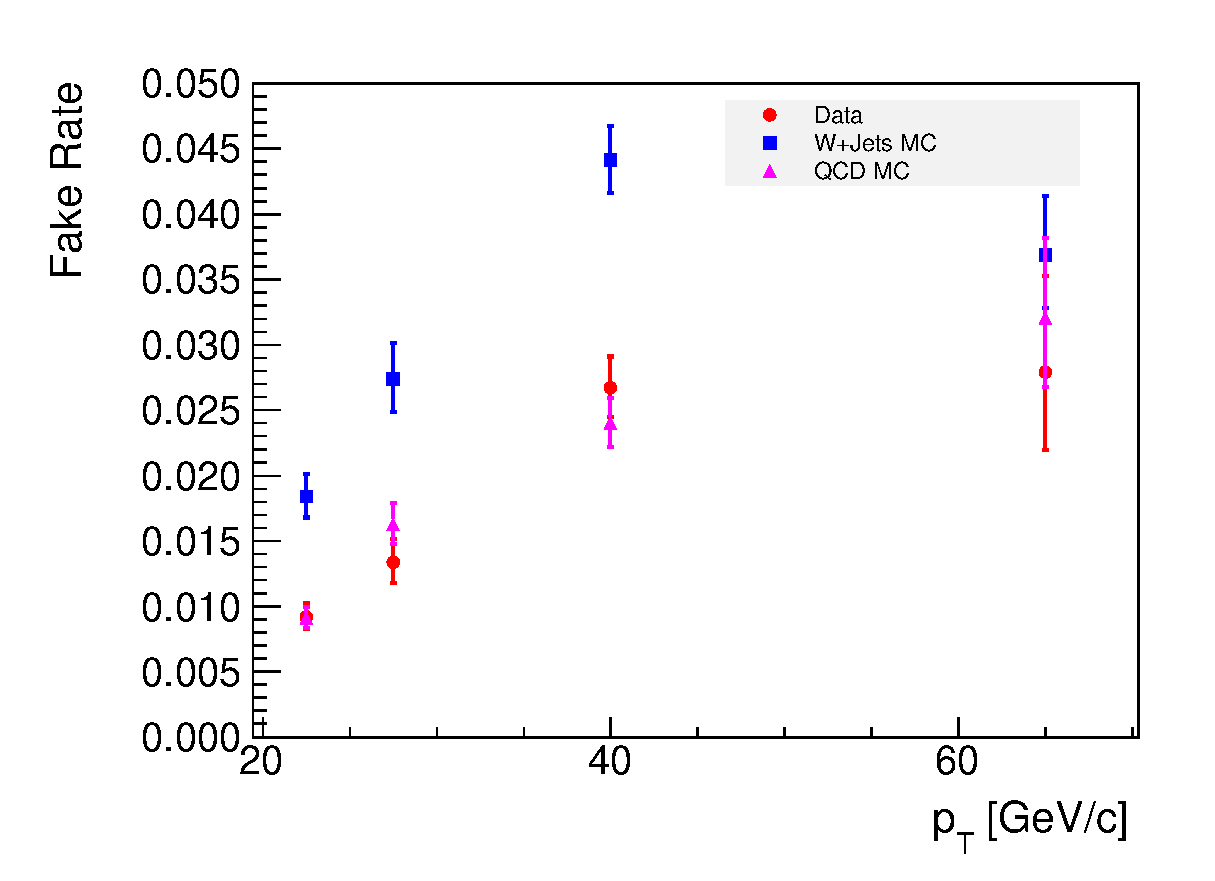
\includegraphics[width=0.49\textwidth]{RecoElectronEfficiency_RecoDenominator_VBTF95WPIdIsoNumerator_Pt.eps}} 
    \subfigure[]{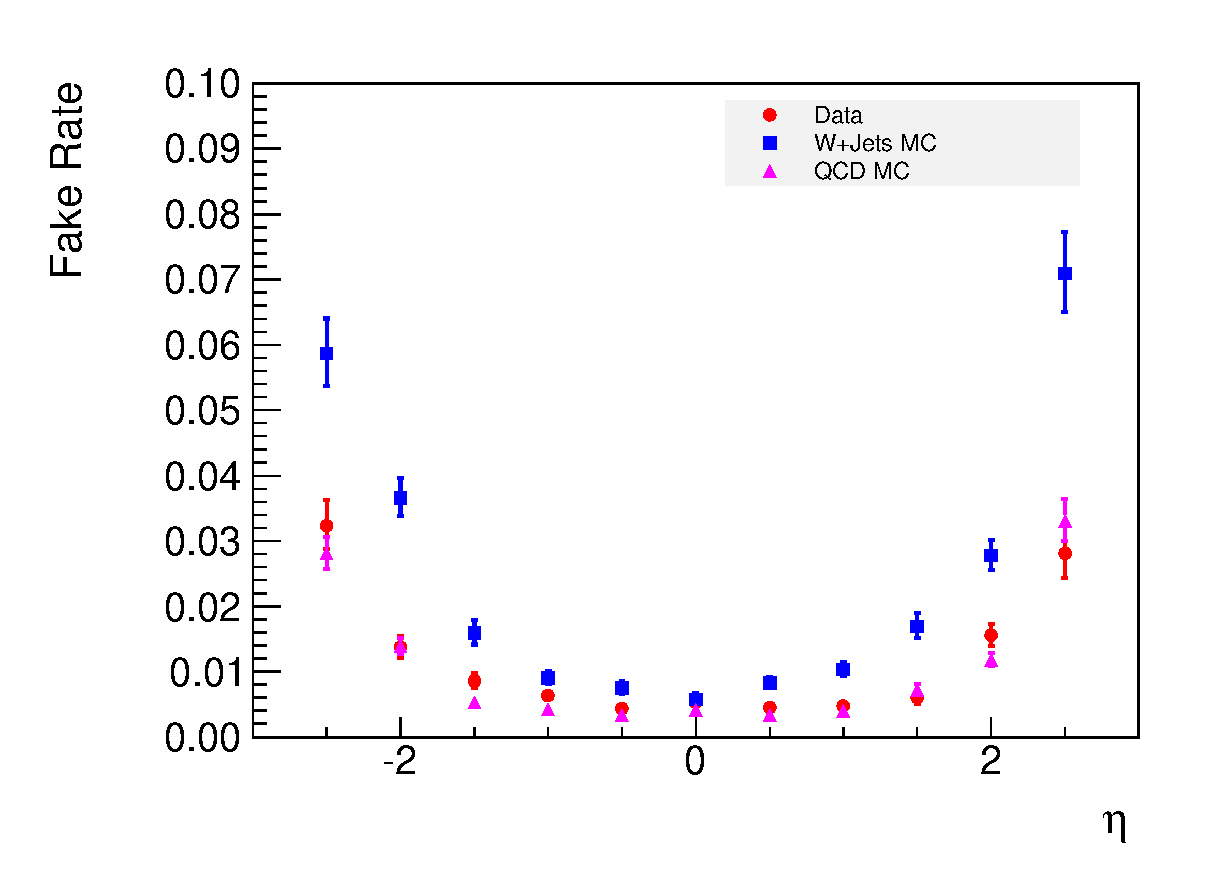
\includegraphics[width=0.49\textwidth]{RecoElectronEfficiency_RecoDenominator_VBTF95WPIdIsoNumerator_Eta.eps}}
    
    \caption{The fake rate for a GSF electron to pass the VBTF95 electron selection measured in the Jet30 data sample are compared to the measurements performed in the corresponding QCD Monte Carlo sample. They are shown as a function of the $p_T$ (a) and $\eta$ (b) of the GSF electron. }
    \label{fig:GSFElectronFakeRate}
  \end{center}
\end{figure}

\begin{figure}[htb]
  \begin{center} 
    \subfigure[GSF electron $p_{T}$ $20$ - $25$]{\includegraphics[width=0.24\textwidth]{ElectronFakeRate_RecoDenominator_VBTF95WPIdIsoNumerator_PtSlices_Pt20.00To25.00.eps}} 
    \subfigure[GSF electron $p_{T}$ $25$ - $30$]{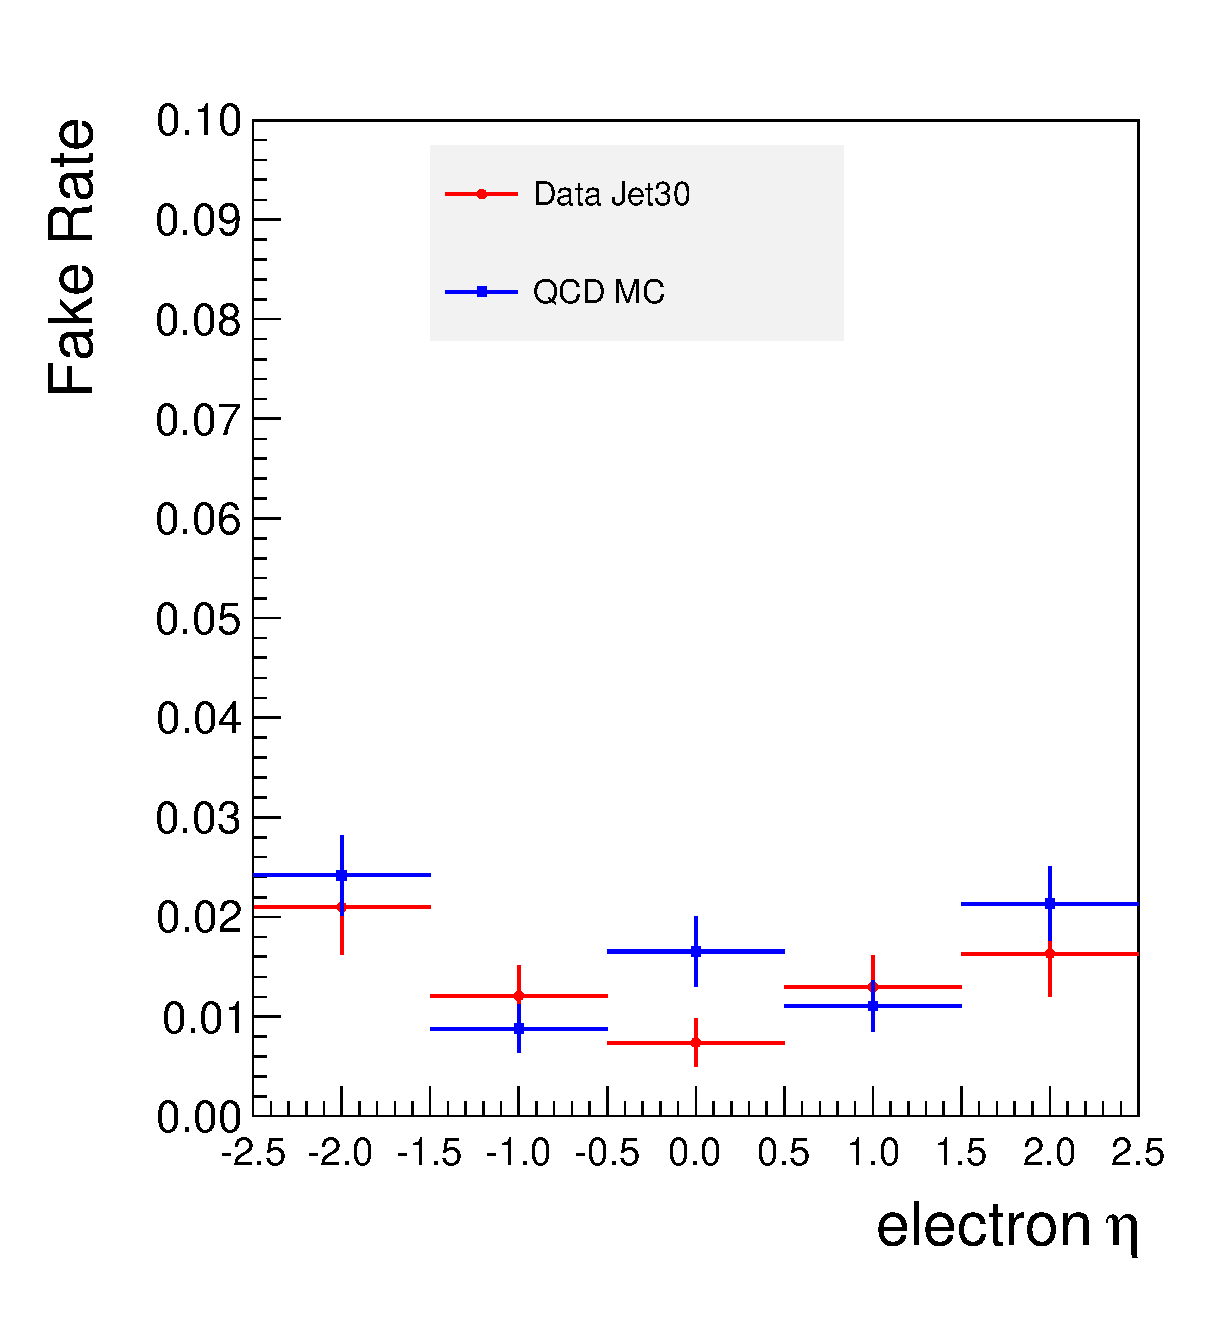
\includegraphics[width=0.24\textwidth]{ElectronFakeRate_RecoDenominator_VBTF95WPIdIsoNumerator_PtSlices_Pt25.00To30.00.eps}}
    \subfigure[GSF electron $p_{T}$ $30$ - $50$]{\includegraphics[width=0.24\textwidth]{ElectronFakeRate_RecoDenominator_VBTF95WPIdIsoNumerator_PtSlices_Pt30.00To50.00.eps}} 
    \subfigure[GSF electron $p_{T}$ $50$ - $80$]{\includegraphics[width=0.24\textwidth]{ElectronFakeRate_RecoDenominator_VBTF95WPIdIsoNumerator_PtSlices_Pt50.00To80.00.eps}}
    
    \caption{The fake rate for a GSF electron to pass the VBTF95 electron selection measured in the Jet30 data sample are compared to the measurements performed in the corresponding QCD Monte Carlo sample. They are shown as a function of $\eta$ in various bins of transverse momentum. }
    \label{fig:GSFElectronFakeRate_slices}
  \end{center}
\end{figure}




One dimensional projections of the fake rate for jets to pass the VBTF95 electron selection are shown in Figure \ref{fig:JetElectronFakeRate} as a function of the transverse momentum and pseudorapidity of the jet. Figure \ref{fig:JetElectronFakeRate_slices} show various slices of the two dimensional fake rate in bins of the transverse momentum. The measurement in the Jet30 data is in close agreement with the prediction from the QCD Monte Carlo simulation, while there is a clear difference with respect to the W+Jets Monte Carlo. This difference is attributed to different fake electron composition and different quark-gluon content, and accounted for in the systematic uncertainties.

\begin{figure}[htb]
  \begin{center}
    \subfigure[]{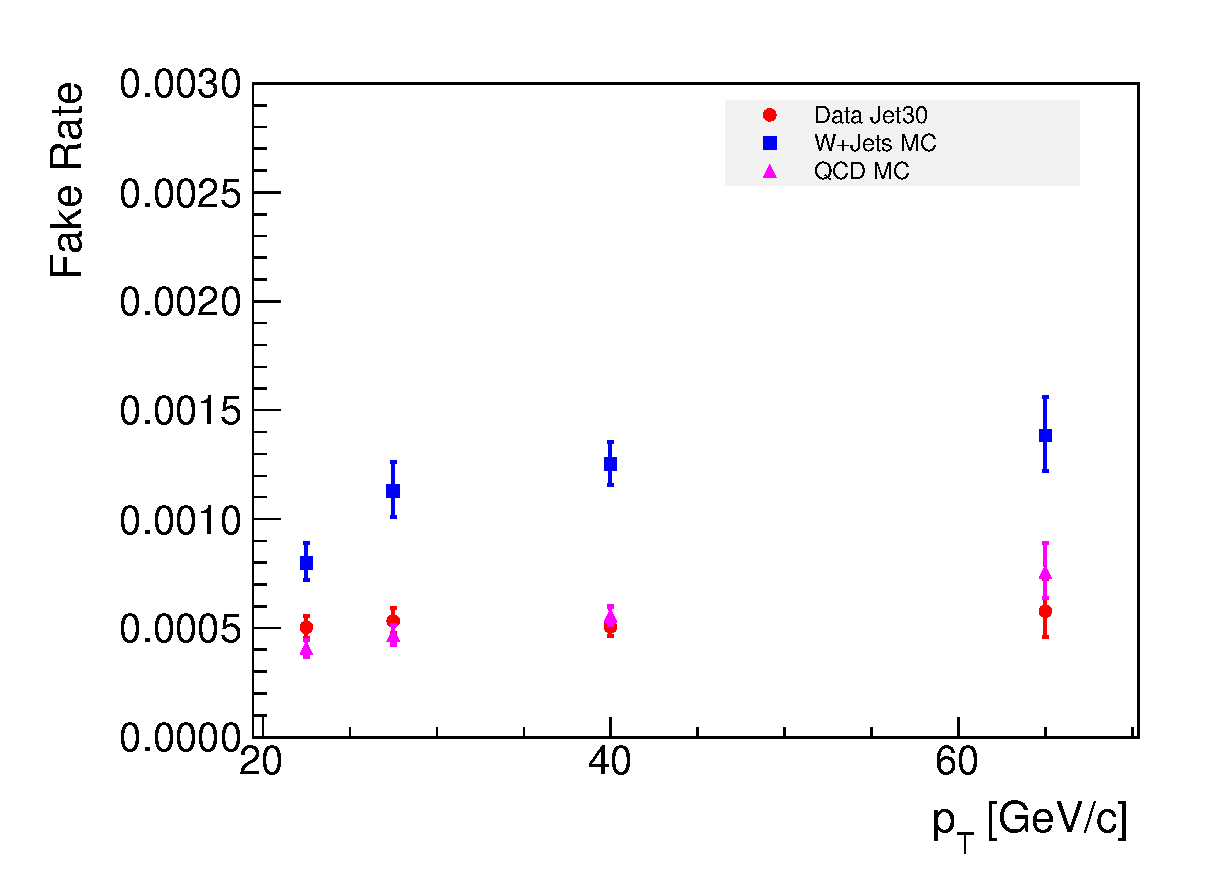
\includegraphics[width=0.49\textwidth]{RecoElectronEfficiency_JetDenominator_VBTF95WPIdIsoNumerator_Pt.eps}} 
    \subfigure[]{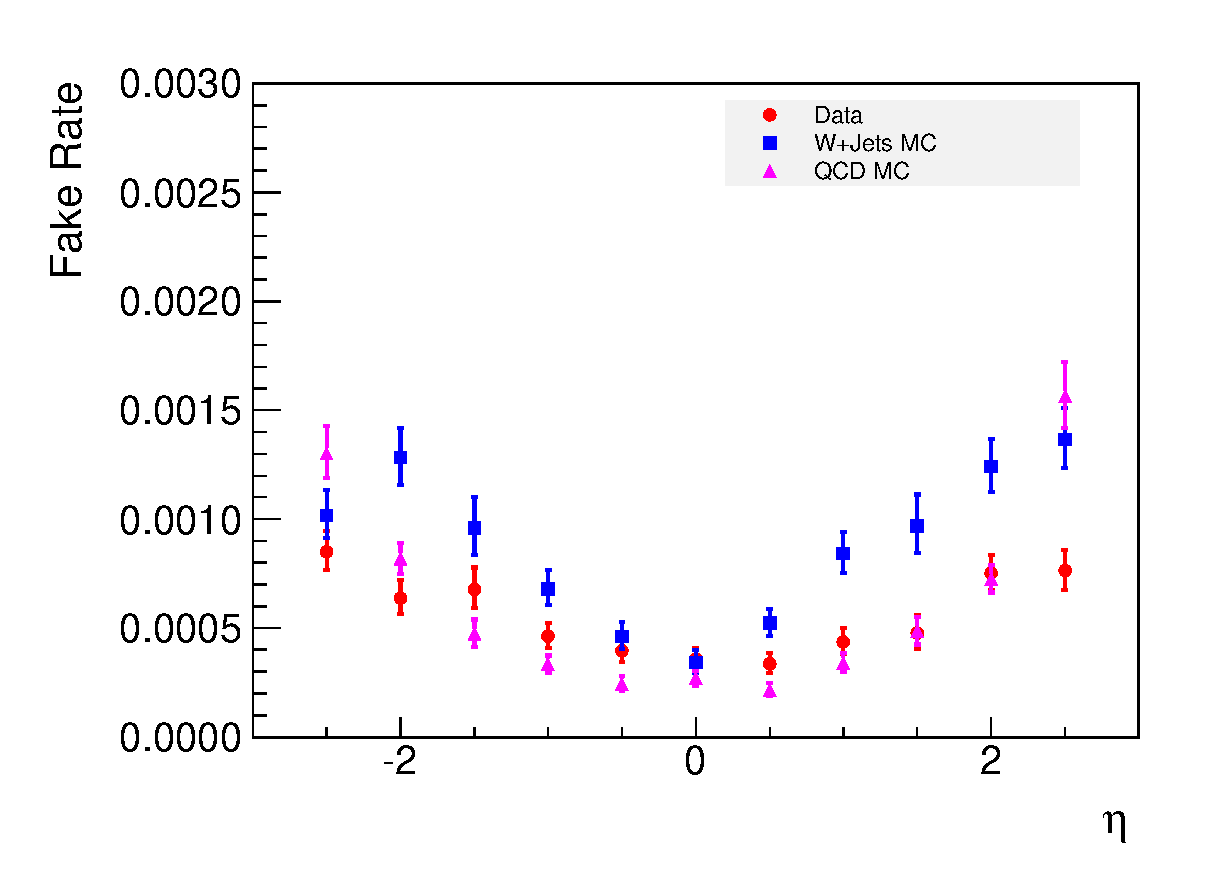
\includegraphics[width=0.49\textwidth]{RecoElectronEfficiency_JetDenominator_VBTF95WPIdIsoNumerator_Eta.eps}}
    
    \caption{The fake rate for a jet to pass the VBTF95 electron selection measured in the Jet30 data sample are compared to the measurements performed in the corresponding QCD Monte Carlo sample. They are shown as a function of the $p_T$ (a) and $\eta$ (b) of the GSF electron. }
    \label{fig:JetElectronFakeRate}
  \end{center}
\end{figure}

\begin{figure}[htb]
  \begin{center}
    \subfigure[jet $p_{T}$ $20$ - $25$]{\includegraphics[width=0.24\textwidth]{ElectronFakeRate_JetDenominator_VBTF95WPIdIsoNumerator_PtSlices_Pt20.00To25.00.eps}} 
    \subfigure[jet $p_{T}$ $25$ - $30$]{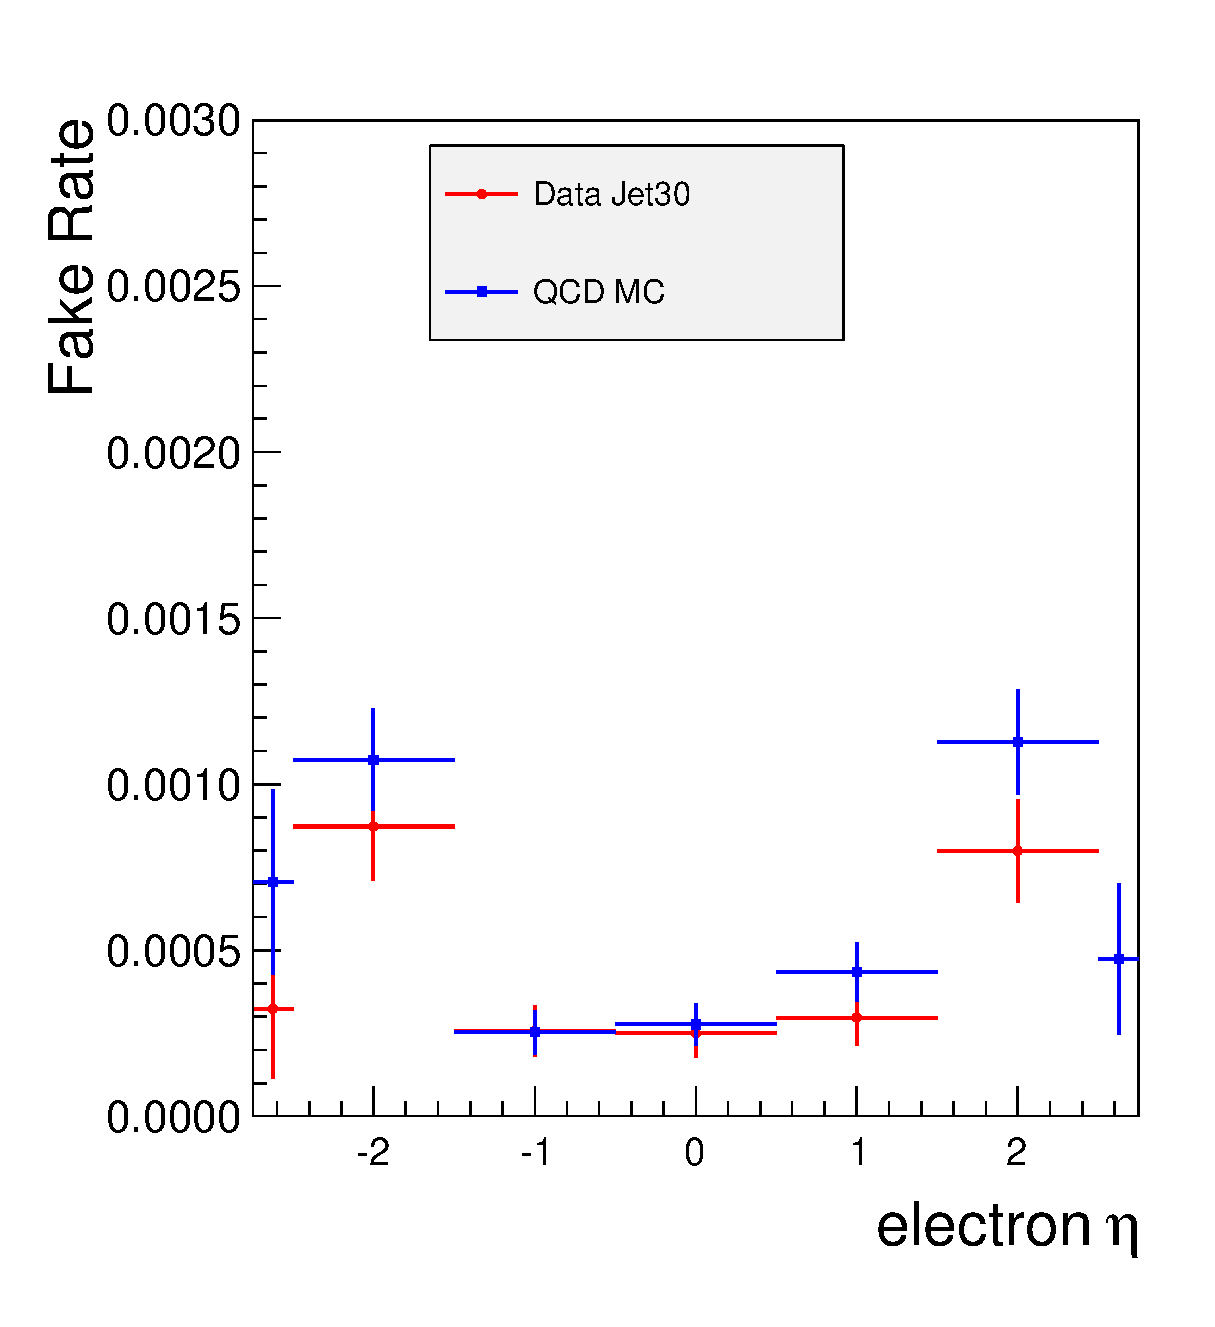
\includegraphics[width=0.24\textwidth]{ElectronFakeRate_JetDenominator_VBTF95WPIdIsoNumerator_PtSlices_Pt25.00To30.00.eps}}
    \subfigure[jet $p_{T}$ $30$ - $50$]{\includegraphics[width=0.24\textwidth]{ElectronFakeRate_JetDenominator_VBTF95WPIdIsoNumerator_PtSlices_Pt30.00To50.00.eps}} 
    \subfigure[jet $p_{T}$ $50$ - $80$]{\includegraphics[width=0.24\textwidth]{ElectronFakeRate_JetDenominator_VBTF95WPIdIsoNumerator_PtSlices_Pt50.00To80.00.eps}}
    
    \caption{The fake rate for a jet to pass the VBTF95 electron selection measured in the Jet30 data sample are compared to the measurements performed in the corresponding QCD Monte Carlo sample. They are shown as a function of $\eta$ in various bins of transverse momentum. }
    \label{fig:JetElectronFakeRate_slices}
  \end{center}
\end{figure}


\customSection{Performance on Monte Carlo Simulation}

We first perform a check of the method using the Monte Carlo simulation, where we apply fake rates computed in simulated QCD events on simulated QCD, W+Jets, and Photon+Jets events and compare the estimate with the prediction of the Monte Carlo simulation. For the QCD simulation prediction, a different Monte Carlo sample has been used where certain generator level cuts have been introduced in order to enhance the number of simulated events with fake electrons. Figures \ref{fig:ZeeQCDBkgPrediction_MC}, \ref{fig:ZeeWJetsBkgPrediction_MC}, and \ref{fig:ZeePhotonJetsBkgPrediction_MC} show the comparison of the estimation using the fake rate method and the simulation prediction as a function of the dielectron mass, for the QCD, and W+Jets and \GAM+Jets background respectively. One observes agreement to within the total uncertainties of the method for the QCD background. The W+Jets background is underestimated due to the fact that the fake rate in W+Jets events is higher than the fake rate in QCD events due to different fake electron composition seen in Figure \ref{fig:JetElectronFakeRate}. This difference is included in the final systematic uncertainty estimate. Figure \ref{fig:ZeeTotalFakeBkgPrediction_MC} shows the analogous comparison for the sum of all fake lepton backgrounds. The resulting predictions for the number of background events in the $60$ GeV to $120$ GeV mass window is shown in Table \ref{tab:mcPrediction} for each of the relevent background processes separately. 



\begin{figure}[htb]
\begin{center}
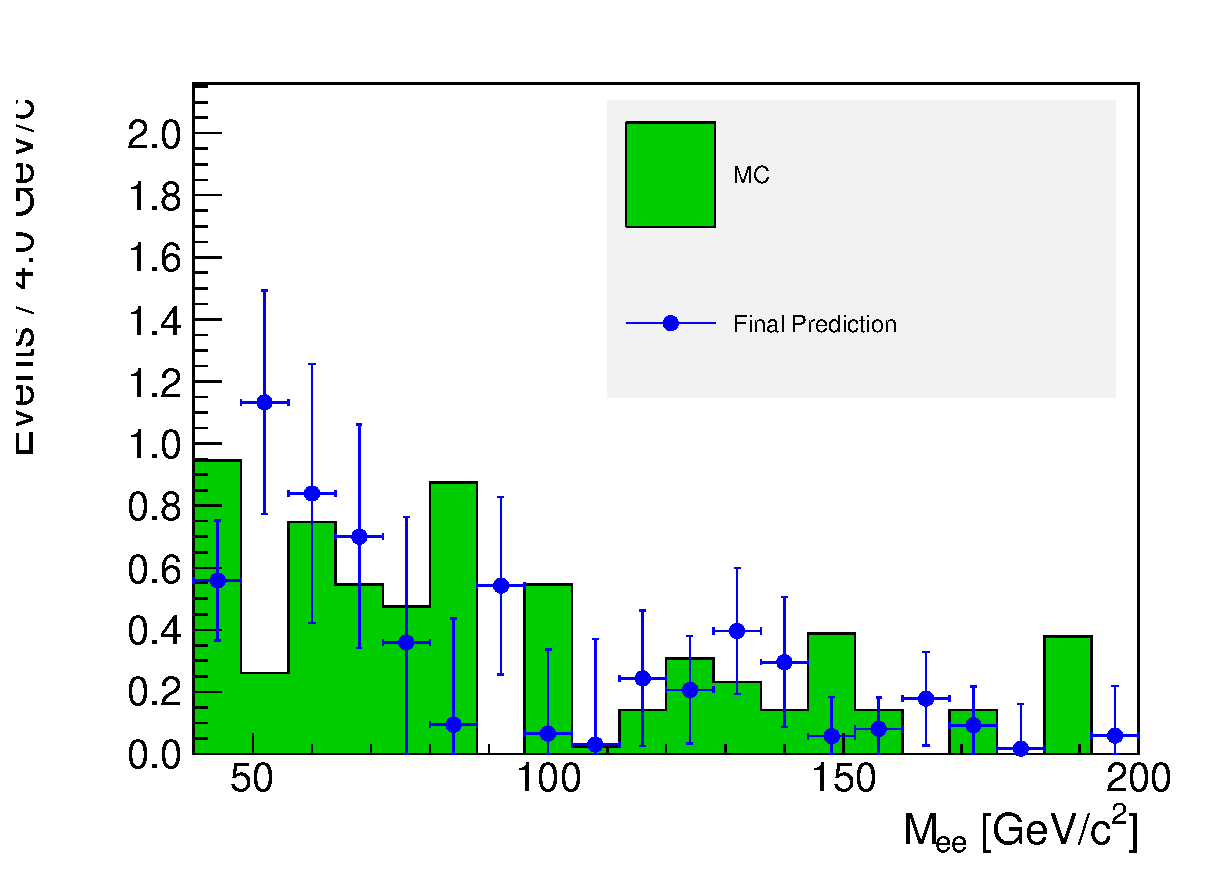
\includegraphics[width=0.49\textwidth]{MCBkgFakeRatePrediction_QCD_FinalVsMC.eps}
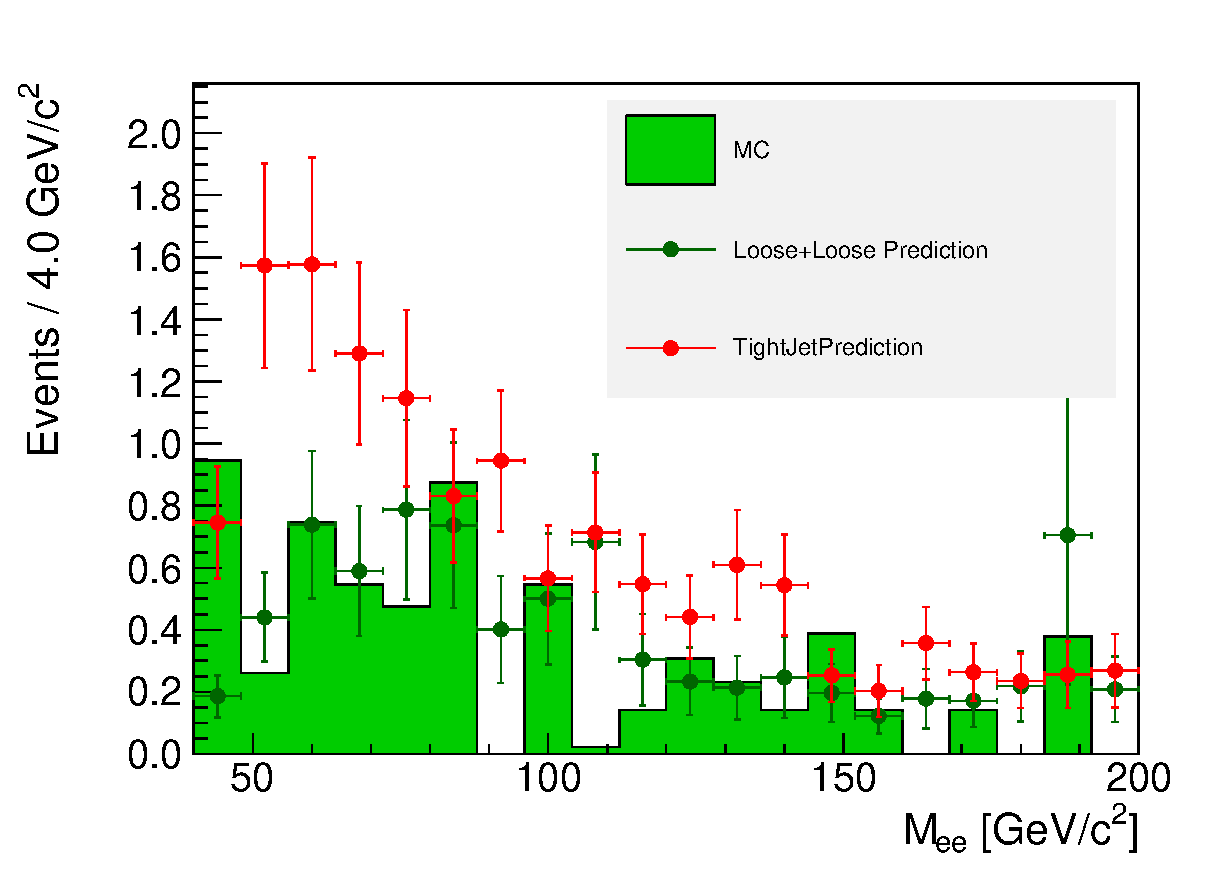
\includegraphics[width=0.49\textwidth]{MCBkgFakeRatePrediction_QCD_LooseLooseTightJetVsMC.eps}
   \caption{The QCD background prediction using the Tight+Jet and Loose+Loose extrapolation performed on Monte Carlo simulation is compared with the direct prediction from the simulation in (a). The Tight+Jet and Loose+Loose extrapolations are compared to the prediction from the simulation in (b). }
   \label{fig:ZeeQCDBkgPrediction_MC}
\end{center}
\end{figure}

\begin{figure}[htb]
\begin{center}
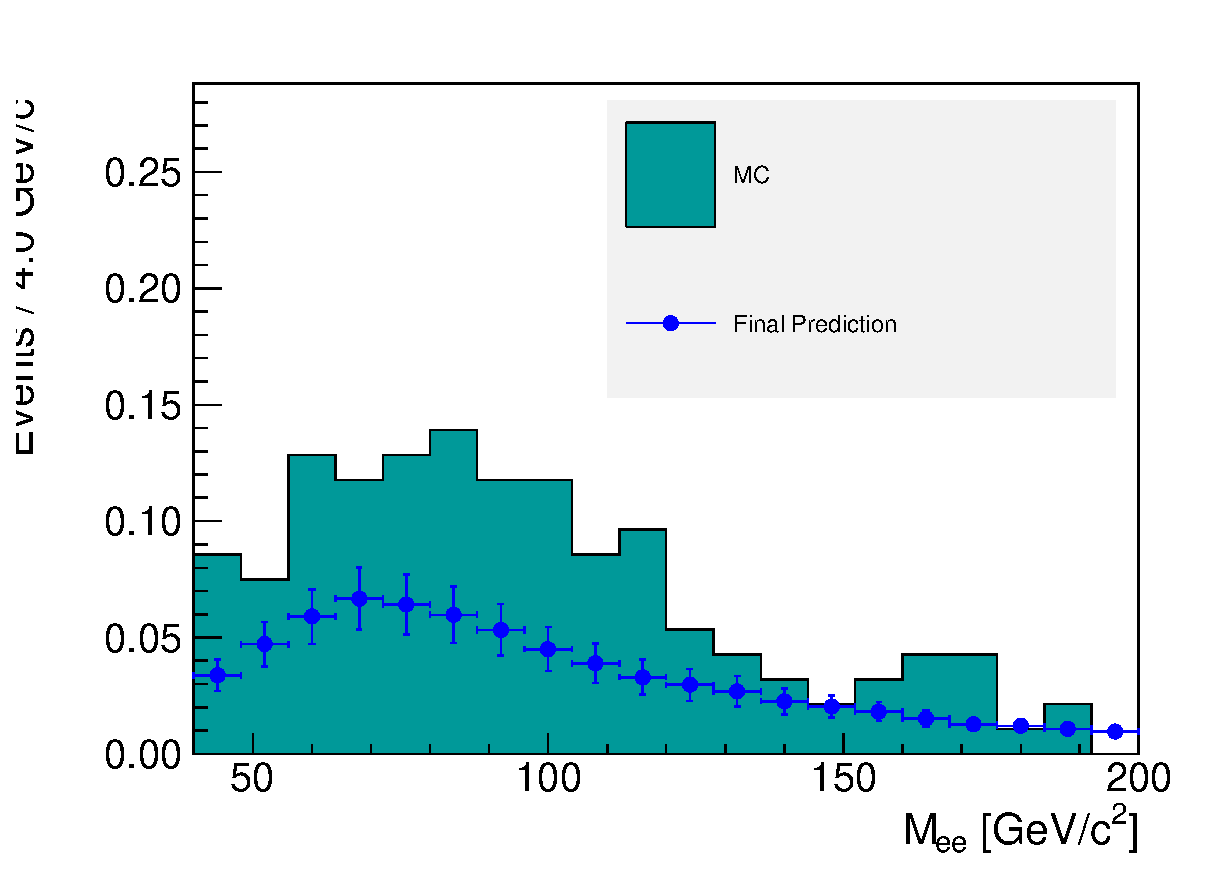
\includegraphics[width=0.49\textwidth]{MCBkgFakeRatePrediction_WJets_FinalVsMC.eps}
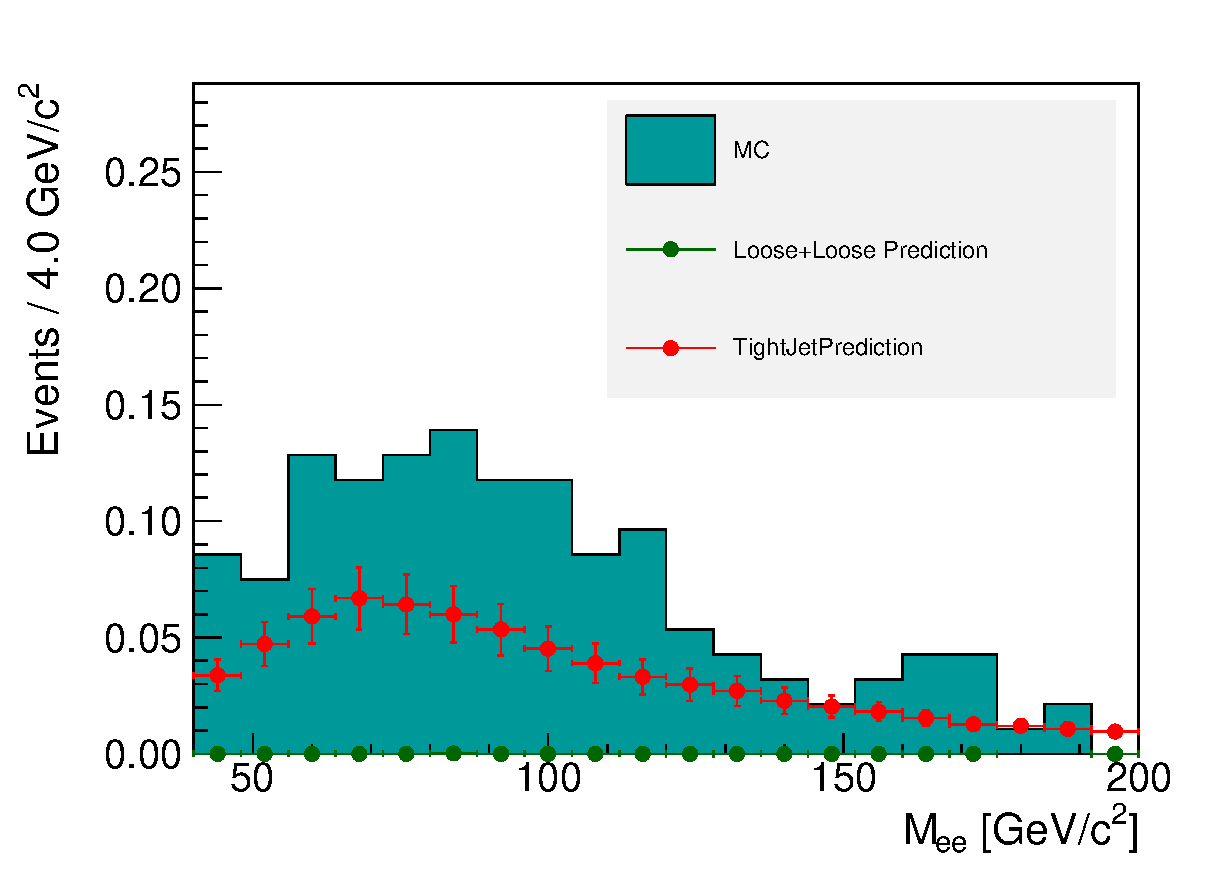
\includegraphics[width=0.49\textwidth]{MCBkgFakeRatePrediction_WJets_LooseLooseTightJetVsMC.eps}
   \caption{The QCD background prediction using the Tight+Jet and Loose+Loose extrapolation performed on Monte Carlo simulation is compared with the direct prediction from the simulation in (a). The Tight+Jet and Loose+Loose extrapolations are compared to the prediction from the simulation in (b). }
   \label{fig:ZeeWJetsBkgPrediction_MC}
\end{center}
\end{figure}

\begin{figure}[htb]
\begin{center}
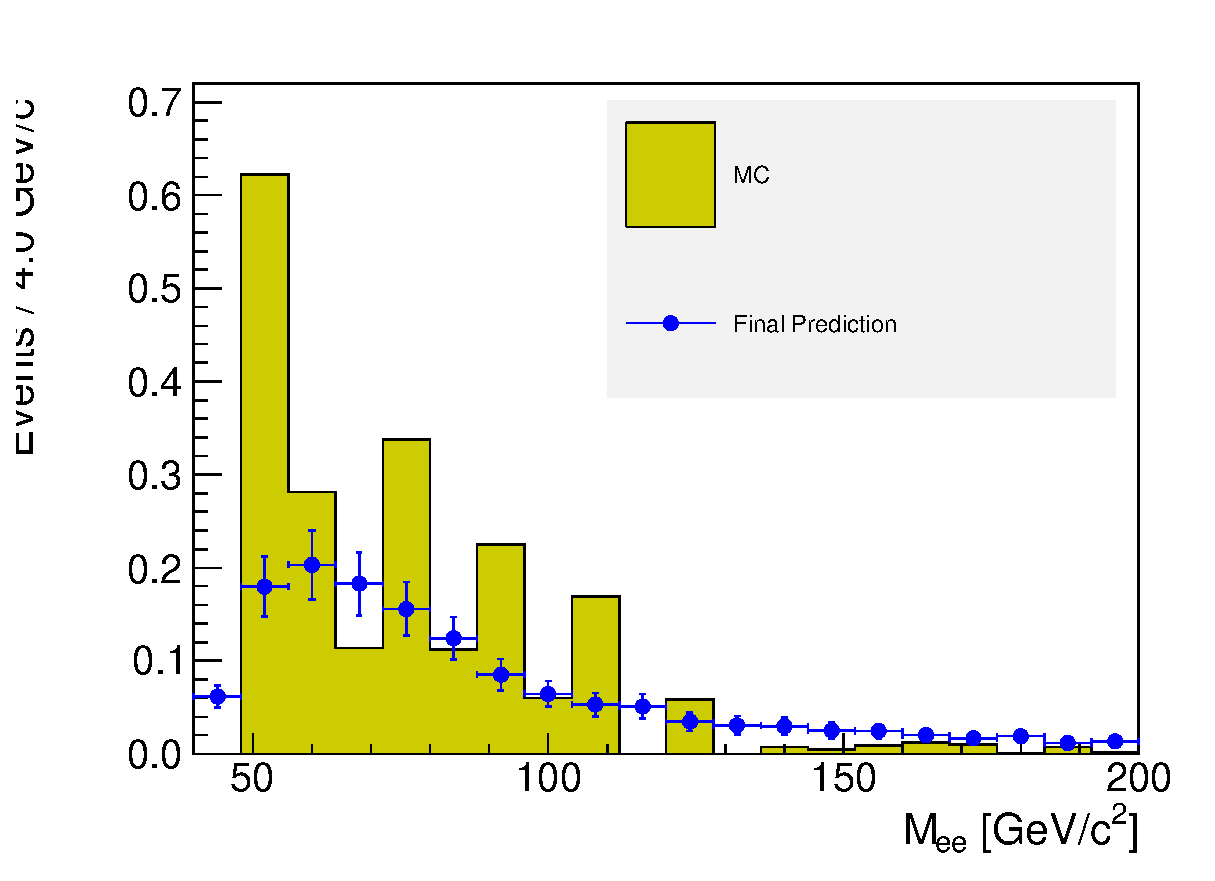
\includegraphics[width=0.49\textwidth]{MCBkgFakeRatePrediction_PhotonJets_FinalVsMC.eps}
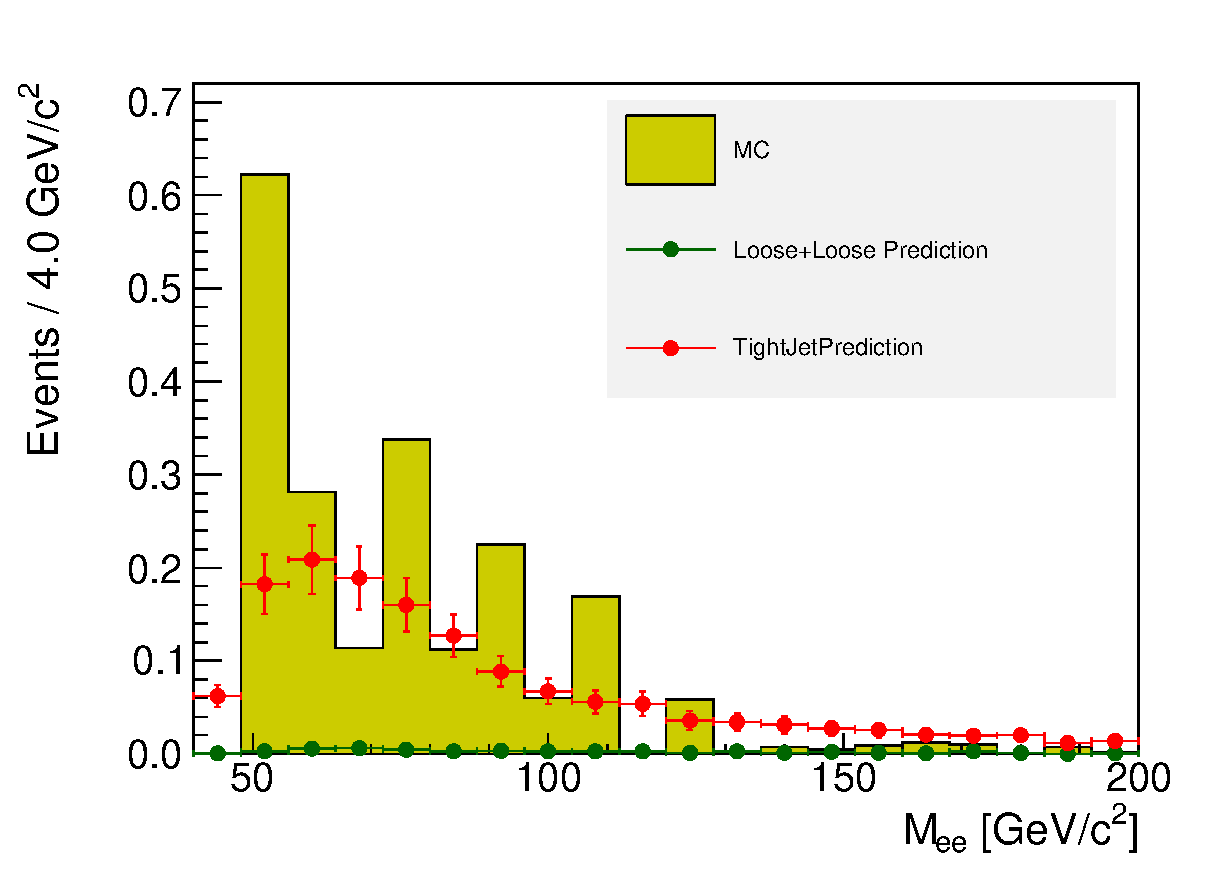
\includegraphics[width=0.49\textwidth]{MCBkgFakeRatePrediction_PhotonJets_LooseLooseTightJetVsMC.eps}
   \caption{The QCD background prediction using the Tight+Jet and Loose+Loose extrapolation performed on Monte Carlo simulation is compared with the direct prediction from the simulation in (a). The Tight+Jet and Loose+Loose extrapolations are compared to the prediction from the simulation in (b). }
   \label{fig:ZeePhotonJetsBkgPrediction_MC}
\end{center}
\end{figure}



\begin{figure}[htb]
\begin{center}
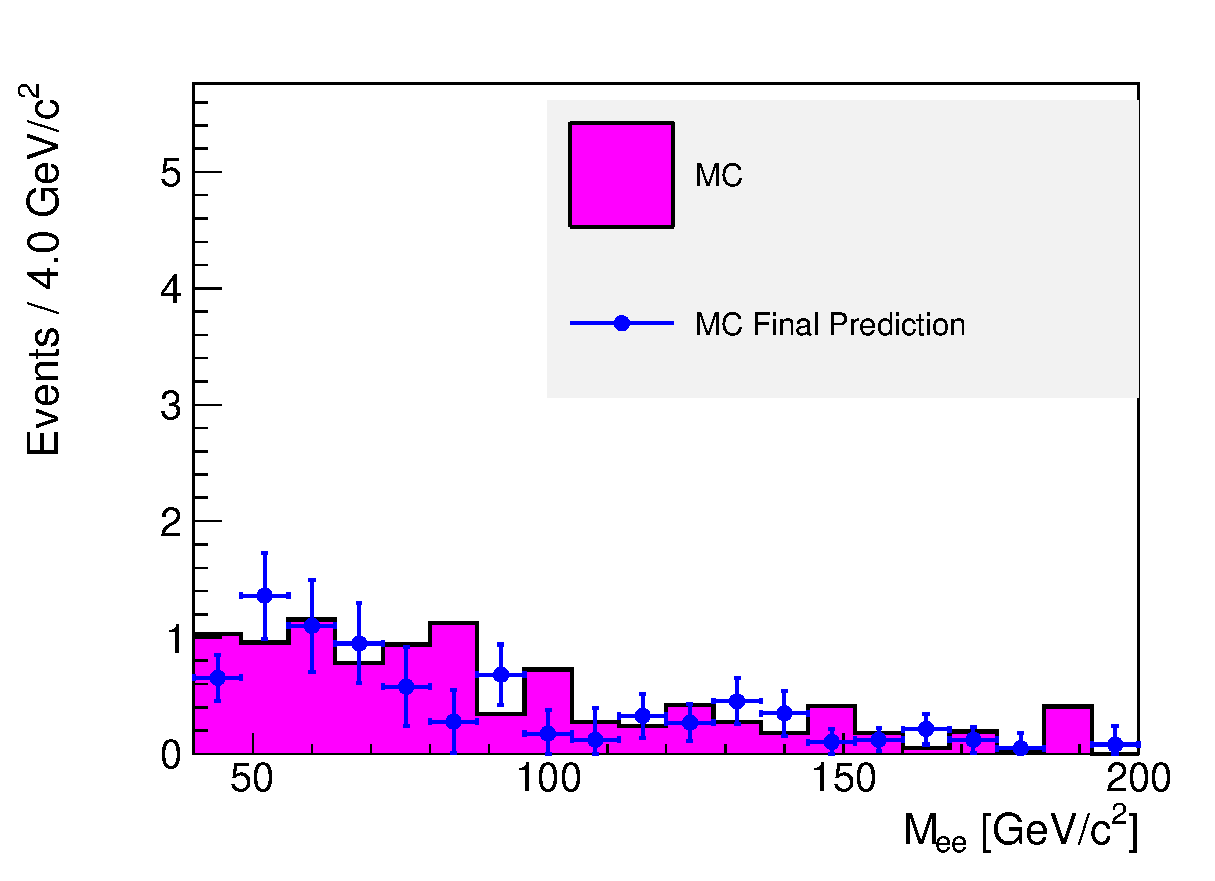
\includegraphics[width=0.49\textwidth]{MCFakeRatePrediction_FinalVsMC.eps}
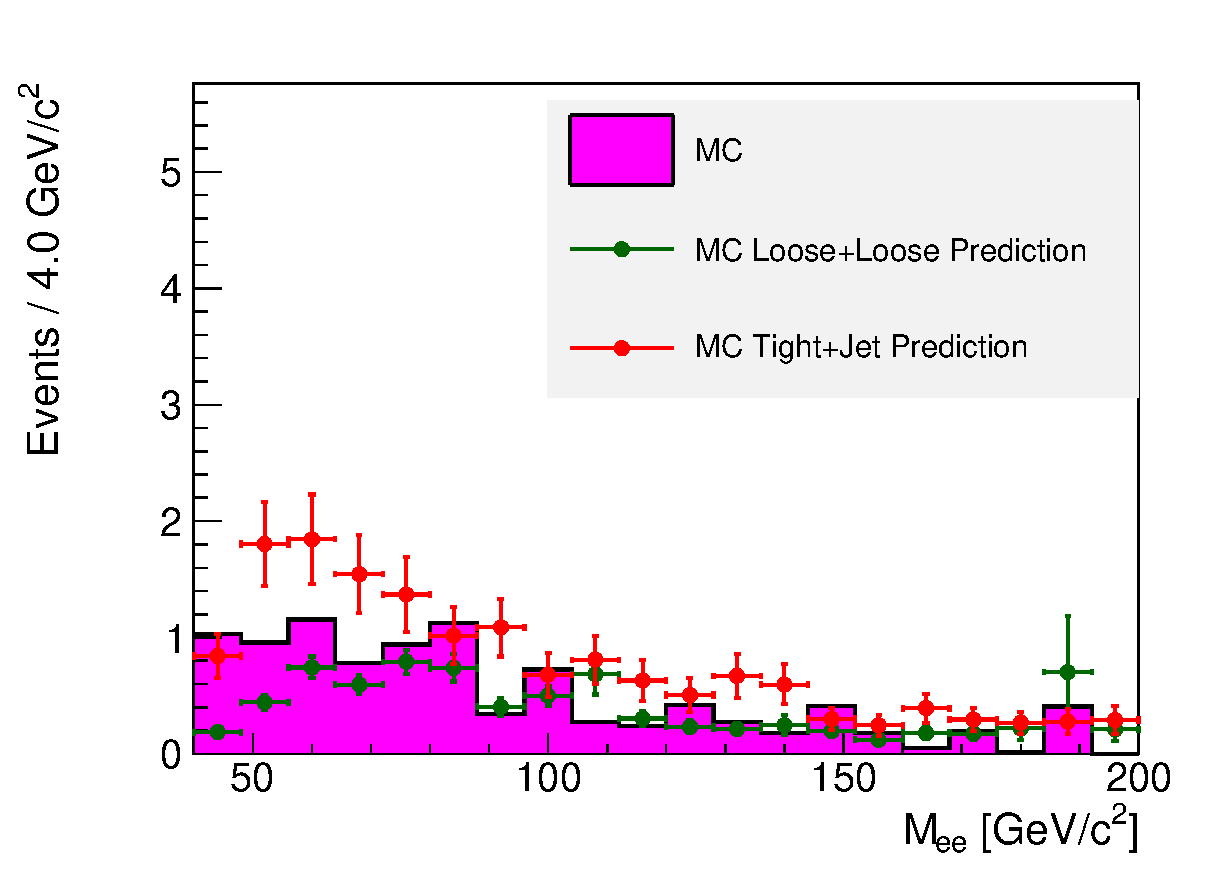
\includegraphics[width=0.49\textwidth]{MCFakeRatePrediction_LooseLooseTightJetVsMC.eps}
   \caption{As a consistency check, the total fake lepton background prediction derived from the fake rate method performed on Monte Carlo simulation is compared with the direct prediction from the simulation in (a), while the Tight+Jet and Loose+Loose extrapolations are separately compared to the simulation prediction in (b). }
   \label{fig:ZeeTotalFakeBkgPrediction_MC}
\end{center}
\end{figure}

The effect of signal contamination on these predictions are estimated by performing the extrapolation procedure on signal Monte Carlo. Figure \ref{fig:ZeeSignalContamination} shows the amount of signal contamination in the Loose+Loose and Tight+Jet predictions compared to the total fake lepton background. The contamination is on the order of $1\%$ for the Tight+Jet prediction and $0.01\%$ for the Loose+Loose prediction. This yields a negligible effect on the final background estimate. 

\begin{figure}[htb]
\begin{center}
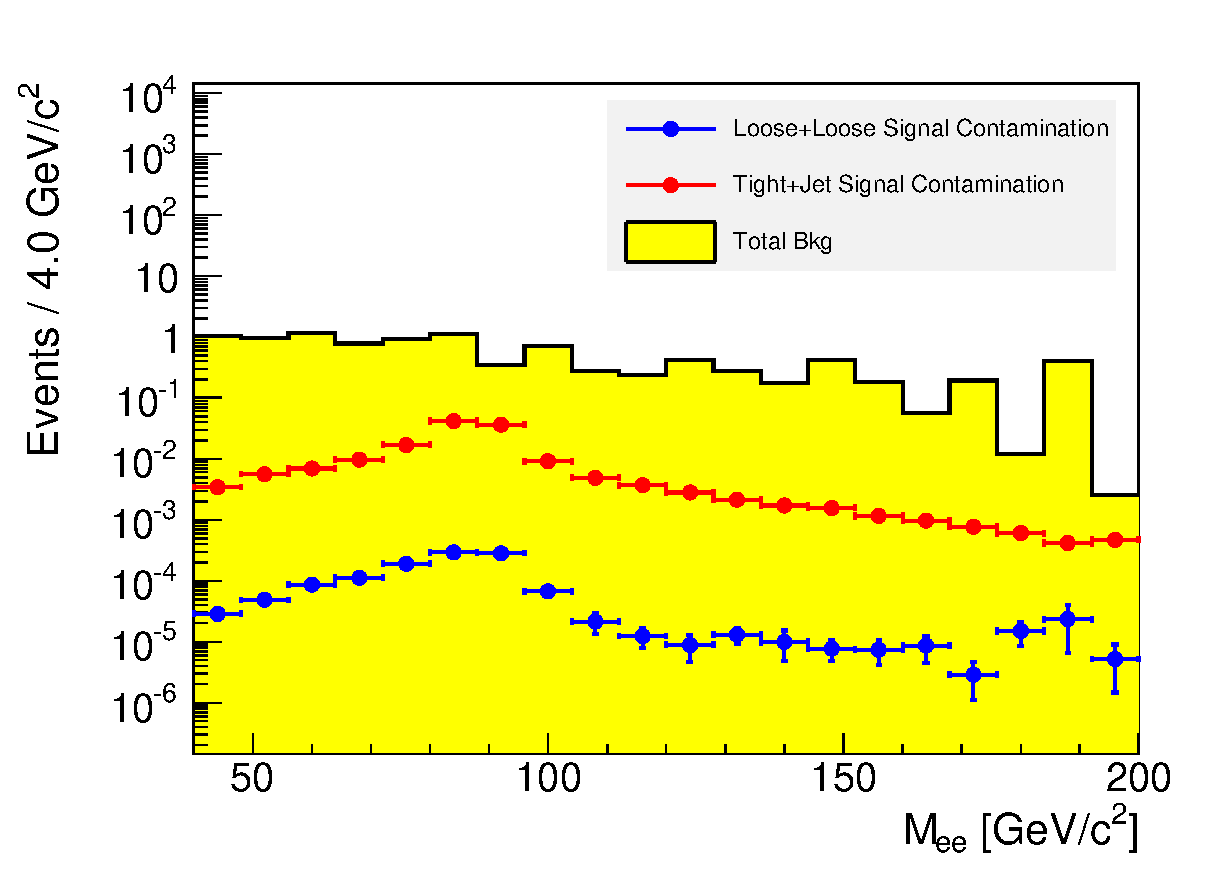
\includegraphics[width=0.49\textwidth]{SignalFakeRateContamination_LooseLooseTightJetVsMCBkg.eps}
   \caption{The signal contamination from \Z\To\EE events in the Tight+Jet and Loose+Loose background prediction calculated from Monte Carlo simulation is compared with the total background prediction. }
   \label{fig:ZeeSignalContamination}
\end{center}
\end{figure}


\begin{table}[!ht]
\begin{center}
\begin{tabular}{|c|c|c|c|c|}
\hline
 Background Process                  &  Tight+Jet Prediction  & Loose+Loose Prediction  & Final Prediction & MC Simulation Prediction \\
\hline
 QCD                                 & 8.1                    & 5.0                     & 3.1              & 3.7                     \\ 
 W+Jets                              & 0.5                    & 0.001                   & 0.5              &  1.0                    \\ 
 Photon+Jets                         & 1.0                    & 0.03                    & 1.0              & 1.4                     \\ 
\hline
 Total                               & 9.5                    & 5.0                     & 4.5              & 6.0                     \\ 
\hline
\end{tabular}
\caption{The predictions obtained from the fake rate method performed on the Monte Carlo are compared with the direct Monte Carlo simulation prediction for each of the relevent background processes separately. \label{tab:mcPrediction}}
\end{center}
\end{table}



\customSection{Data Results}

The data driven estimate of the fake lepton background is compared to the prediction from the Monte Carlo simulation in Figure \ref{fig:ZeeTotalFakeBkgPrediction_Data}. The Tight+Jet and Loose+Loose predictions are also separately compared to the background predicted by the Monte Carlo simulation. The background estimate inside the Z mass window is summarized in Table \ref{tab:dataPrediction}, along with the uncertainties. 

\begin{figure}[htb]
\begin{center}
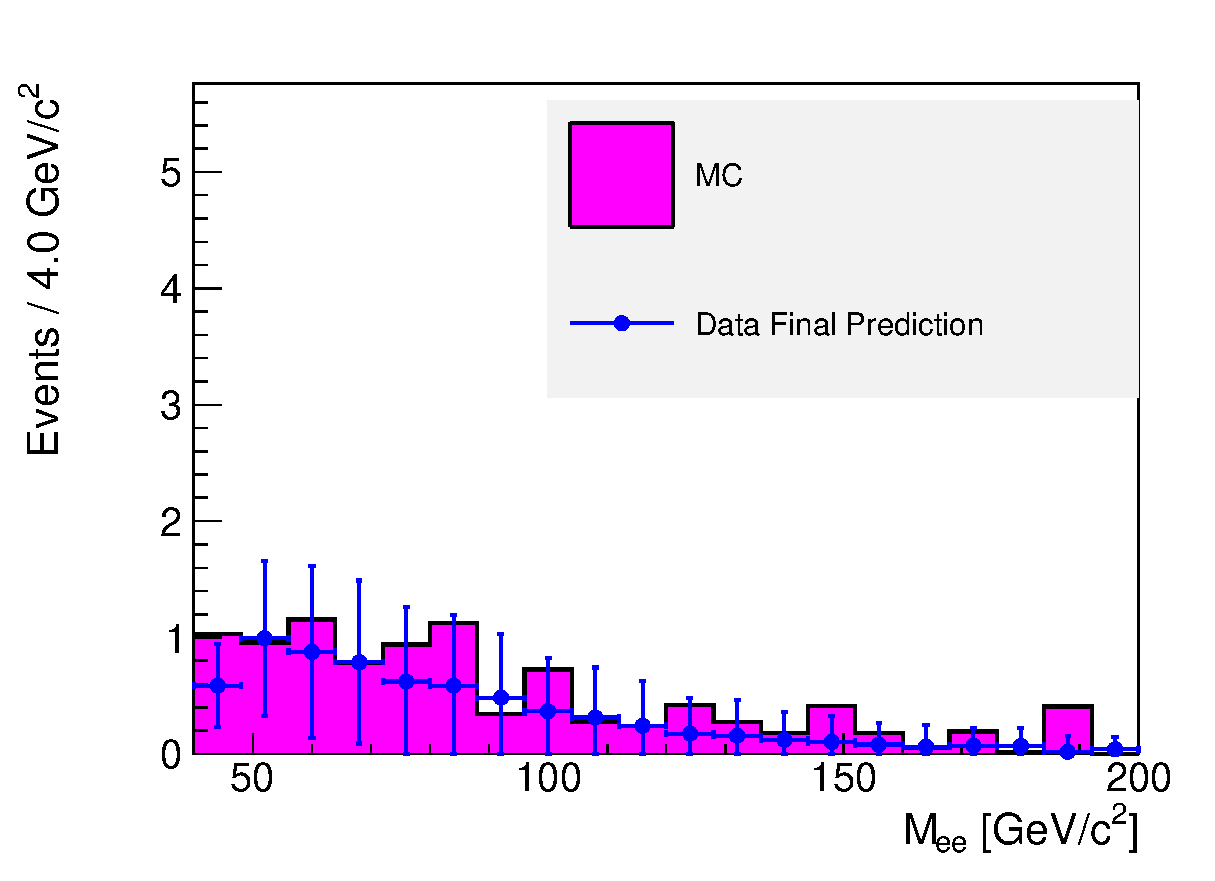
\includegraphics[width=0.49\textwidth]{FakeRatePrediction_FinalVsMC.eps}
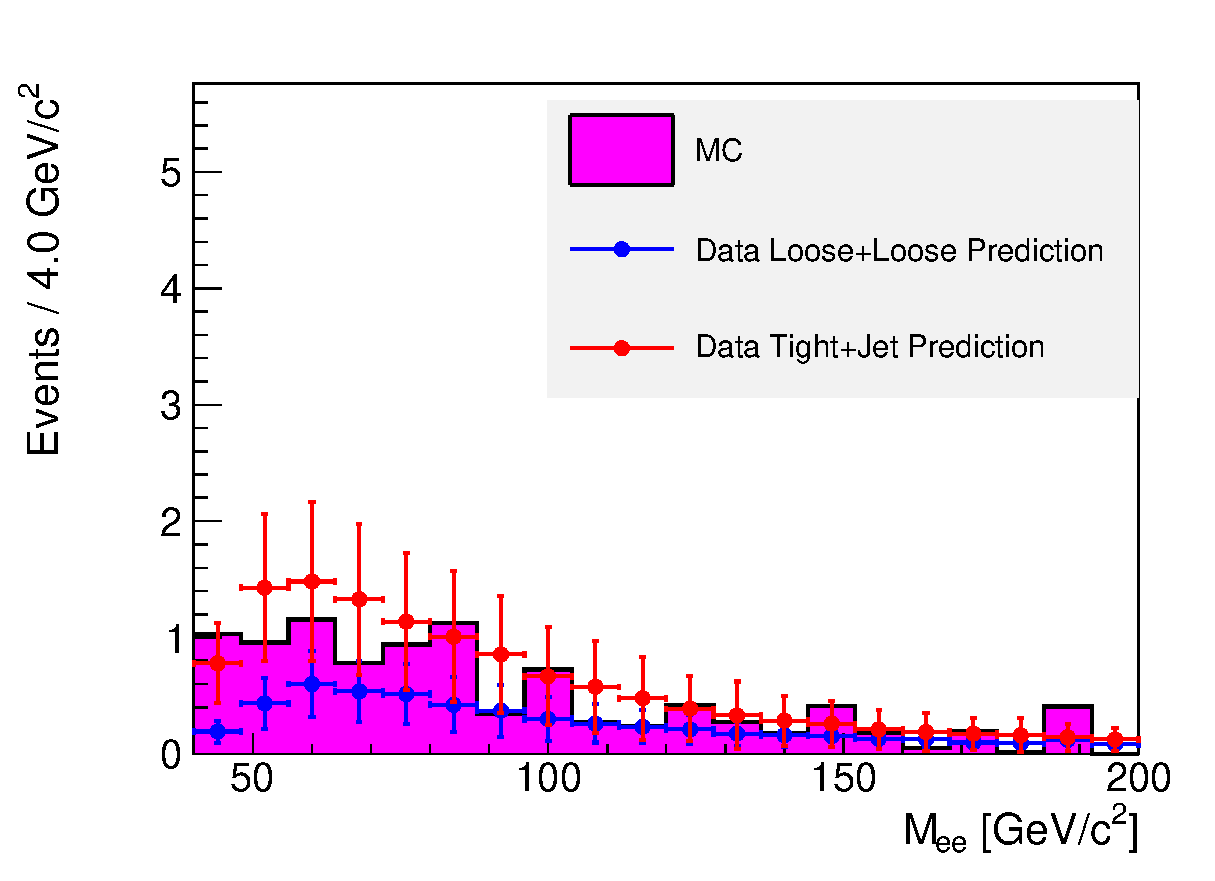
\includegraphics[width=0.49\textwidth]{FakeRatePrediction_LooseLooseTightJetVsMC.eps}
   \caption{The data driven fake lepton background prediction is compared with the prediction from the Monte Carlo simulation in (a), while the Tight+Jet and Loose+Loose extrapolations from data are separately compared with the prediction from the Monte Carlo simulation in (b). }
   \label{fig:ZeeTotalFakeBkgPrediction_Data}
\end{center}
\end{figure}


\begin{table}[!ht]
\begin{center}
\begin{tabular}{|c|c|}
\hline
 Data Tight+Jet Events               & 15820 \\
 Tight+Jet Prediction                & 7.9 +- 4.7 (stat) +- 2.2 (W+Jets systematics) \\
\hline
 Data Loose+Loose Events             & 13906 \\
 Loose+Loose Prediction              & 3.5 +- 2.0 (stat) \\
\hline
 Final Prediction                    & 4.5 +- 5.1 (stat) +- 2.2 (W+Jets systematics) \\
\hline
 MC Simulation Prediction            & 6.0 +- 0.9 \\
\hline
\end{tabular}
\caption{The data driven fake lepton background estimates are summarized and compared to the result from the MC simulation. Only statistical uncertainties are given and dominated by the statistical uncertainty of the binned fake rate measurements. \label{tab:dataPrediction}}
\end{center}
\end{table}



\customSection{Systematic Uncertainties}

The dominant systematic uncertainties are those associated with the fake rate measurement itself. There may be differences between the calibration sample and the dielectron sample, in both the composition of the exact fake processes, each with different fake rates, and in the amount of jet activity, which affects the isolation fake rate. 

To account for the difference in jet activity, we take the difference between the Jet30 data measurement and the Jet15 data measurement as a systematic uncertainty. However, the comparison, shown in Figures \ref{fig:RecoFakeRateJetTriggerSystematics} and \ref{fig:JetFakeRateJetTriggerSystematics}, yields a negligible difference. 

To account for the composition effect, we take the difference between the fake rate measurement from the Jet30 data measurement and the W+Jet fake rate from Monte Carlo as a systematic uncertainty for the fraction of the background that originate from W+Jets and \GAM+Jets events. This fraction is calculated from the Tight+Jet and Loose+Loose predictions as in equation \ref{eqn:WJetRatioFormula} and found to be roughly $0.2$ in data. 

\begin{eqnarray}
  \label{eqn:WJetRatioFormula}  
\mathrm{Fraction\ of\ non-QCD\ Background} = 1 - \frac{N_{\mathrm{Loose+Loose}}}{N_{\mathrm{Tight+Jet}} - N_{\mathrm{Loose+Loose}}}
\end{eqnarray}

This difference between the W+Jets fake rate and the fake rate measured in the Jet30 data is illustrated in Figure \ref{fig:JetElectronFakeRate} for the jet fake rate.  This systematic uncertainty is only included for the Tight+Jet extrapolation because the Loose+Loose prediction does not account for any W+Jets background by construction. When propagated to the Tight+Jet prediction, we obtain a systematic uncertainty of $2.2$ events.

\begin{figure}[htb]
  \begin{center}
    \subfigure[]{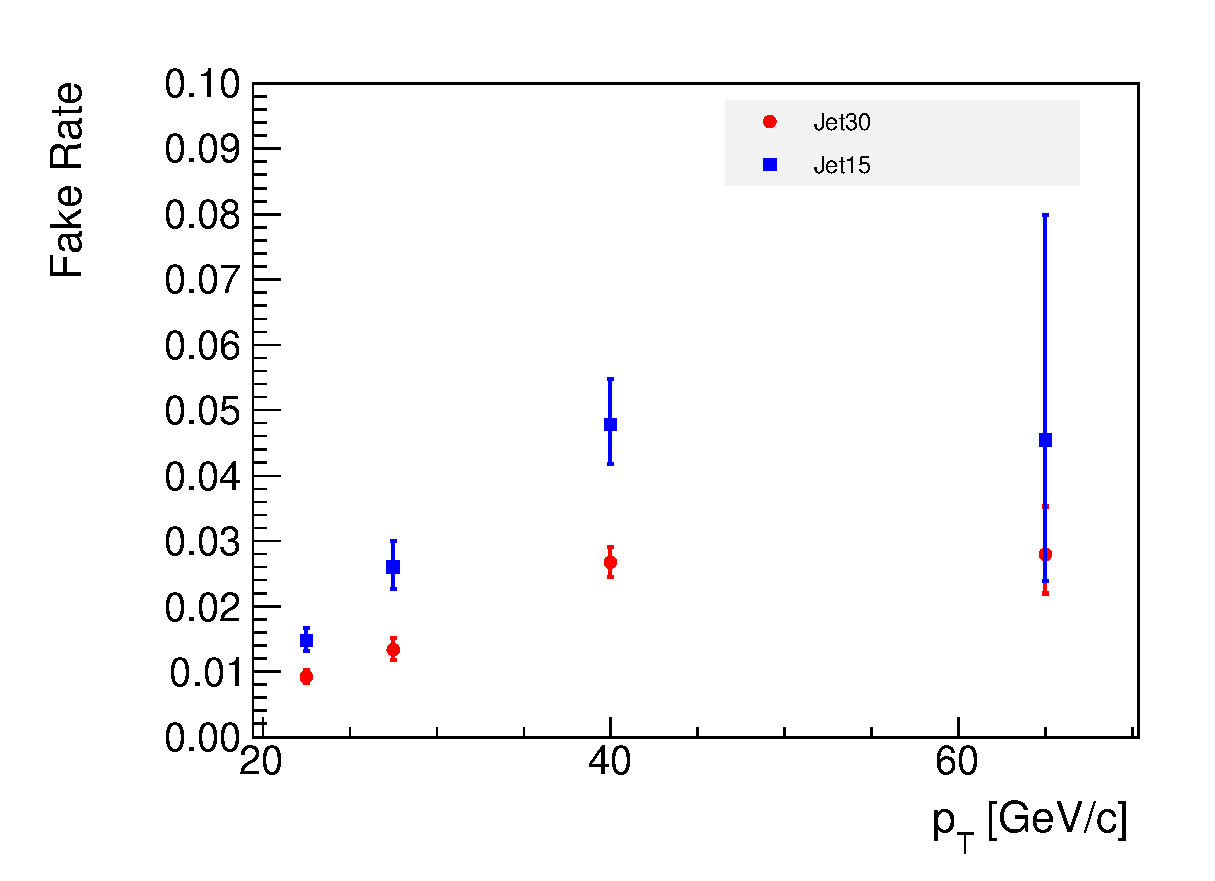
\includegraphics[width=0.49\textwidth]{RecoElectronEfficiency_RecoDenominator_VBTF95WPIdIsoNumerator_JetTriggerSystematics_Pt.eps}}     
    \caption{A comparison is made between the fake rate for GSF electrons to pass VBTF95 electron selection ($\epsilon_{\mathrm{fake}}$) measured in the Jet30 data sample and the Jet15 data sample.}
    \label{fig:RecoFakeRateJetTriggerSystematics}
  \end{center}
\end{figure}

\begin{figure}[htb]
  \begin{center}
    \subfigure[]{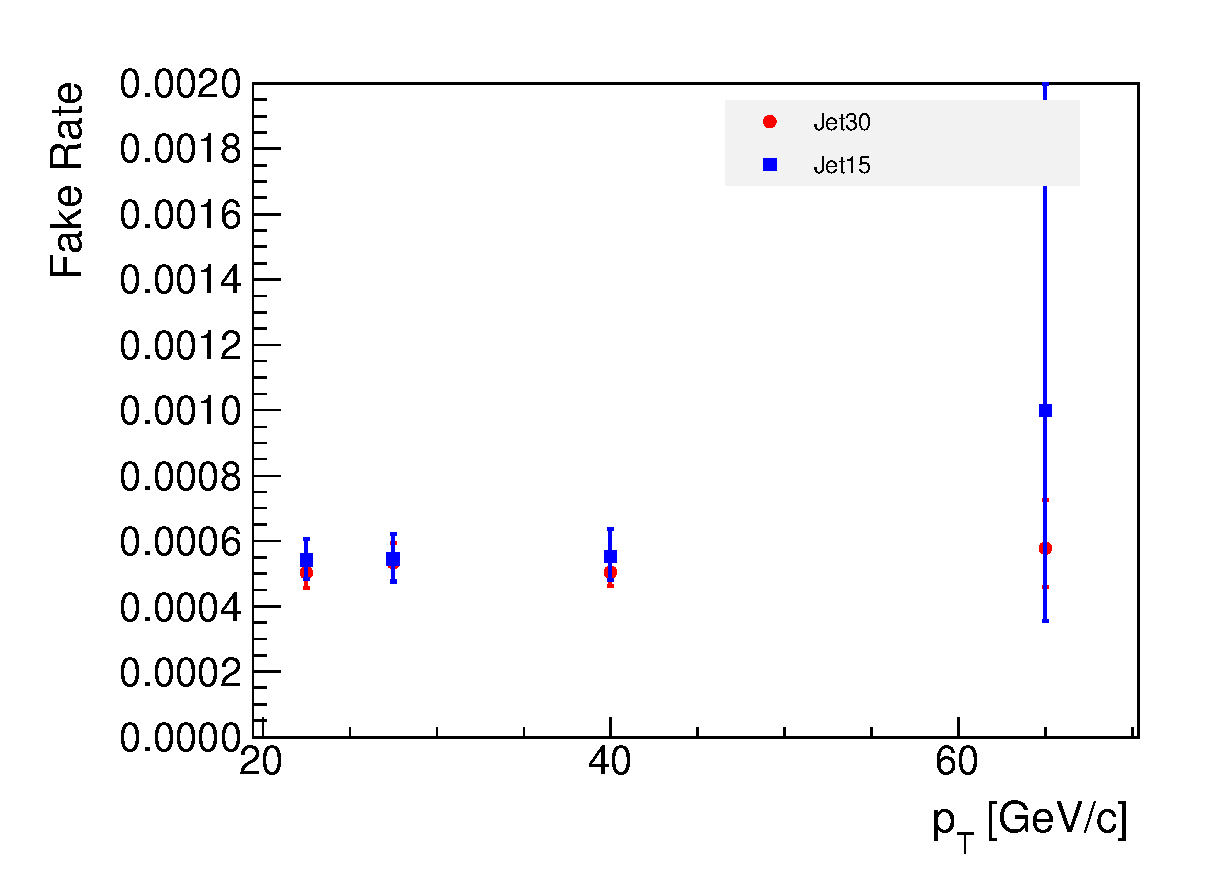
\includegraphics[width=0.49\textwidth]{RecoElectronEfficiency_JetDenominator_VBTF95WPIdIsoNumerator_JetTriggerSystematics_Pt.eps}}     
    \caption{A comparison is made between the fake rate for jets to be matched to a GSF electron passing the VBTF95 electron selection ($\epsilon_{\mathrm{fake}}$) measured in the Jet30 data sample and the Jet15 data sample.}
    \label{fig:JetFakeRateJetTriggerSystematics}
  \end{center}
\end{figure}


Finally, an additional systematic uncertainty due to jet angular resolution is considered. Since an electron inside a jet may point significantly away from the central jet axis, it is possible for a jet whose direction is outside of the electron acceptance region in $\eta$ to give a fake electron whose direction points inside the acceptance region. To estimate the magnitude of this effect, we compute the Tight+Jet prediction for jets with $|\eta|$ between $2.5$ and $2.75$. The resulting number of events for the dataset under consideration is $0.3$, which is roughly $7\%$ of the total background estimate. This represents a negligible part of the total systematic uncertainty. 


\customSection{Conclusion}
We have combined two different data driven techniques to estimate the total fake lepton background for the \Z\To\EE analysis in $2.88\ipb$. We estimate a total fake lepton background of $4.5 \pm 5.1$ (statistical) $\pm 2.2$ (systematic) events. A comprehensive set of systematic effects are taken into account and propagated to the final result. The current total uncertainty on the fake lepton background determination using this method represents a roughly $0.6\%$ uncertainty on the \Z\To\EE cross section measurement, dominated by the statistical uncertainty from the measurement of the fake rate in jet data, which will decrease with an increasing data sample. This measurement serves as a supplemental documentation for the main W and Z inclusive cross section measurement described here\cite{UpdatedCrossSectionNote}.



\vspace*{-0.2cm}
\thebibliography{12}

\bibitem{CrossSectionNote}
 CMS AN-2010/116 , ``Measurements of Inclusive W and Z Cross Sections in pp Collisions at $\sqrt{s}=7$ TeV'', 
The Vector Boson Task Force of the CMS Collaboration  \textit{et al.}.

\bibitem{FakeRateNote}
 CMS AN-2009/120, ``Study of Data-Driven Methods For Estimation of Fake Lepton Backgrounds'',
G. Bauer \textit{et al.}.

\bibitem{UpdatedCrossSectionNote}
 CMS AN-2010/264 , ``Updated Measurements of Inclusive W and Z Cross Sections at $\sqrt{s}=7$ TeV'', 
J. Alcaraz Maestre, \textit{et al.}.


\end{document}


